\documentclass{article}

% Packages
\usepackage[utf8]{inputenc}
\usepackage[T1]{fontenc}
\usepackage[
a4paper,
headheight=20mm,% Set \headheight to 10mm
bottom=3cm
]{geometry}
\usepackage{layout}
\usepackage{lipsum}
% AMS style packages
\usepackage{amsfonts}
\usepackage{amsmath}
%\usepackage{amsrefs}
\usepackage{amssymb}
\usepackage{amstext}
\usepackage{amsthm}
\usepackage{array}

%money stuff
\usepackage{textcomp}
\usepackage{eurosym}

%noindent
\usepackage{parskip}

\usepackage[table]{xcolor}

% Standard useful packages
\usepackage[shortlabels]{enumitem}
\usepackage{float}
\usepackage{graphicx}
\usepackage{mathrsfs}
\usepackage{multicol}
\usepackage{wasysym}
\usepackage{caption}
\usepackage{subcaption}
\usepackage{url}
\usepackage{csquotes}

% algorithms
\usepackage{algorithm}
\usepackage{algpseudocode}

% tableau bayésiens
\usepackage{booktabs}
\usepackage{multirow}

% Font warnings
\usepackage{silence}
\WarningFilter{latexfont}{Font shape}
% Tikz package and libraries
\usepackage{tikz}
\usepackage{tikz-cd}
%\usepackage{tikzducks}
\usetikzlibrary{arrows, backgrounds, calc, chains, decorations, patterns, positioning, shapes, arrows.meta}

% pstricks
\usepackage{pstricks}
\usepackage{pstricks-add}

%nicematrix
\usepackage{nicematrix}

%svg
\usepackage[inkscapeformat=png]{svg}

% tableau stylés
\usepackage{mathtools, nccmath, hhline}
\usepackage{makecell}
\setcellgapes{3pt}

% Environments
\theoremstyle{plain}
\theoremstyle{definition}
\newtheorem{thm}{Theorem}
\newtheorem{conj}{Conjecture}
\newtheorem{cor}{Corollary}
\newtheorem{defi}{Definition}
\newtheorem{lem}{Lemma}
\newtheorem{prop}{Proposition}
\newtheorem{prob}{Problem}
\newtheorem{exo}{Exercise}
\newenvironment{preci}{\textbf{Precision} : }{}
\newenvironment{res}[1][]{\textbf{\underline{Resolution} #1} :\\}{\vspace{.2cm}}{}

\theoremstyle{remark}
\newtheorem{remark}{Remark}
\newtheorem{example}{Example}
\newtheorem*{note}{Note}

\newcommand{\numberwithinenvs}{subsection}

\numberwithin{thm}{\numberwithinenvs}
\numberwithin{conj}{\numberwithinenvs}
\numberwithin{cor}{\numberwithinenvs}
\numberwithin{defi}{\numberwithinenvs}
\numberwithin{lem}{\numberwithinenvs}
\numberwithin{prop}{\numberwithinenvs}
\numberwithin{prob}{\numberwithinenvs}
\numberwithin{exo}{\numberwithinenvs}
\numberwithin{remark}{\numberwithinenvs}
\numberwithin{example}{\numberwithinenvs}

\renewcommand{\qedsymbol}{$\blacksquare$}
\newenvironment{fprf}{\par{\itshape Non-proof.}}{\qed}
\newenvironment{fthm}{{\itshape Non-theorem.}}{\vspace{.2cm}}

% Comments
\usepackage{comment}


%custom titling
\usepackage{titling}
\newcommand{\seance}[1]{\newcommand{\theseance}{#1}}
\newcommand{\authors}[1]{\newcommand{\theauthor}{#1}}
\newcommand{\rapport}[1]{\newcommand{\rapportNb}{#1}}
\newcommand{\synthese}[1]{\newcommand{\syntheseNb}{#1}\thematic{Résumé}}
\newcommand{\thematic}[1]{\newcommand{\theThematic}{#1}}
\newcommand{\mnemonic}[1]{\newcommand{\theMnemonic}{#1}}
\newcommand{\course}[1]{\newcommand{\theCourse}{#1}}
\newcommand{\mytitle}[1]{
    \begin{center}
        \textbf{\LARGE\thetitle}
    \end{center}
    \vspace{.5cm}
}
\newcommand{\mytitlewithauthor}[1]{
    \begin{center}
        \textbf{\LARGE\thetitle}
        \\
        \theauthor
    \end{center}
    \vspace{.5cm}
}


% Custom commands
\newcommand{\NN}{\mathbb{N}}
\newcommand{\ZZ}{\mathbb{Z}}
\newcommand{\QQ}{\mathbb{Q}}
\newcommand{\RR}{\mathbb{R}}
\newcommand{\CC}{\mathbb{C}}
\DeclareMathOperator*{\argmax}{arg\,max}
\DeclareMathOperator*{\argmin}{arg\,min}

\newcounter{Question}
\counterwithin{Question}{section}
\newcommand{\question}[1]{\stepcounter{Question}\vspace*{1em}{\large Q\theQuestion.~\textit{#1}}}

% Header and footer
\usepackage{fancyhdr}
\usepackage{lastpage}
\usepackage[bottom]{footmisc}
\pagestyle{fancy}
\fancyhead[L]{\includegraphics[width=0.2\textwidth]{assets/ulb/ulb}}
\fancyhead[R]{\textsc{\texttt{\theMnemonic}, \texttt{\theThematic}}}
\fancyfoot[C]{\thepage}
%\fancyfoot[L]{\today}
%\fancyfoot[R]{\textsc{\thepage\ / \pageref{LastPage} }}
\renewcommand{\headrulewidth}{0.4pt}
\renewcommand{\footrulewidth}{0pt}


% Listings
\usepackage{listingsutf8}
\usepackage{listings}
\definecolor{backgroundgray}{RGB}{250,250,250}
\definecolor{codegray}{rgb}{0.5,0.5,0.5}
\definecolor{codegray2}{rgb}{0.5,0.5,0.5}
\definecolor{codewriting}{rgb}{0.2,0.2,0.2}

\lstset{
    language=python,
    showspaces=false,
    showstringspaces=false,
    showtabs=false,
    backgroundcolor=\color{backgroundgray},
    commentstyle=\color{codegray2},
    keywordstyle=\bfseries\color{red!50},
    %frame=single,
    aboveskip=12pt,
    belowskip=12pt,
    xleftmargin=12pt,
    xrightmargin=12pt,
    basicstyle=\ttfamily\small\color{codewriting},
    numbers=left,
    numbersep=5pt,
    numberstyle=\tiny\color{codegray},
    literate={é}{{\'e}}1{à}{{\`a}}1{è}{{\`e}}1{ç}{{\c c}}1{~}{{$\sim$}}1{œ}{{\oe}}1
}

% custom figure numbering
\numberwithin{equation}{subsection}
\counterwithin{figure}{section}

% hyperref
\usepackage[colorlinks = true,
            linkcolor = purple,
            anchorcolor = blue,
            citecolor = blue]{hyperref}

% bibliography
\usepackage[numbers]{natbib}
\bibliographystyle{acm}

% \synthese{}
\mnemonic{INFO-H518}
\course{Immersive Multimedia Technologies I}
\thematic{Report}

\title{\texttt{\theMnemonic}: \theCourse \\ \texttt{\theThematic}}
\author{Mathieu Vannimmen \texttt{(543455)}}
\date{\texttt{\today}}

\begin{document}

\maketitle

{\hypersetup{linkcolor=black}
    \tableofcontents
}
\newpage

\section{First Part}\label{sec:firstpart}

    \section{Radial Distortion Removal}\label{sec:radialdistortion}

In the course, we saw that radial distortion can be modeled as follows:
\begin{equation}\label{eq:radialdistortion}
\begin{cases}
    x'&=p_x+(x-p_x)(1+k_1 r^2+k_2 r^4)\\
    y'&=p_y+(y-p_y)(1+k_1 r^2+k_2 r^4)
\end{cases}
\end{equation}
Where the point $(x,y)$ lands in $(x',y')$ in the distorted image, with
$r^2=\left\| (x,y)-(p_x,p_y) \right\|_2^2=(x-p_x)^2+(y-p_y)^2$.
This means that all points $(x,y)$ at an equal distance $d$ from the principal point $p=(p_x,p_y)$ get distorted the
same amount.
Furthermore, only knowing $p$ and $k_1,k_2$ enables one to invert any distortion by inverting
equation~\eqref{eq:radialdistortion}.

\question{How does the algorithm know that it has converged to a good (or good enough) solution?
What is the error function, exactly?}

\question{Try polynomial and division models. Comment on the difference in results.}

\question{Explain the difference in the principal point position between [A] and [B].}

\question{Explain why we see blurry regions in the output result.}

\question{Is the result reliable? Please comment.}

\question{Show which kind of radial distortion you get with positive and negative k-values.}

Let us assume that $p=(0,0)$ is the center of the image plane to simplify computations and consider the line $y=1$.
We are interested in what happens to the $y$ coordinate of a point $(x,1)$ on the line.
By equation~\eqref{eq:radialdistortion}, we have:

\[y'=1+k_1 (x^2+1)+k_2 (x^2+1)^2\]

Taking the derivative, we obtain
\[\frac{dy'}{dx}=2k_1 x+4k_2 x(x^2+1)\]

If $k_1,k_2<0$, we find that $y'$ is increasing for $x<0$ and decreasing for $x>0$.
Hence, we get barrel distortion.
If $k_1,k_2>0$, we find that $y'$ is decreasing for $x<0$ and increasing for $x<0$.
This is pincushion distortion.

Note that with this model, if $k_1$ is of a different sign than $k_2$, we can have that horizontal lines get distorted
in ways that are neither \enquote*{barrel} nor \enquote*{pincushion} (one can picture some arbitrary fourth-degree
polynomial).

    \subsection{Homography for panoramic stitching}\label{subsec:homography}

A homography is a transformation of space that can model a translation, rotation and shear of a picture, as well as a
perspective change.
This is used in the context of panoramic stitching to take two pictures with a common section and stitch them
together (only if the two pictures are taken from the same position or if the photographied scene is planar).

A homography is a $3\times 3$ matrix that maps 2D points in homogeneous coordinates to other 2D points in homogeneous
coordinates.

\begin{equation}\label{eq:homography}
    H=\left[
\begin{array}{c c c}
    h_1 & h_2 & h_3 \\
    h_4 & h_5 & h_6 \\
    h_7 & h_8 & 1
\end{array}
\right]
\end{equation}

If we take a point $X$, $HX=X'$ is where the point is sent by the homography.

\begin{equation}\label{eq:homographyapplication}
    HX=\left[
\begin{array}{c c c}
    h_1 & h_2 & h_3 \\
    h_4 & h_5 & h_6 \\
    h_7 & h_8 & 1
\end{array}
\right]\left[\begin{array}{c}
            x \\ y \\ 1
\end{array}\right]=\left[\begin{array}{c}
            h_1 x + h_2 y + h_3 \\ h_4 x + h_5 y + h_6 \\ h_7 x + h_8 y + 1
\end{array}\right]=X'=\left[
\begin{array}{c}
    x' \\ y' \\ w'
\end{array}\right]
\end{equation}

We can notice in equation~\eqref{eq:homographyapplication} that $h_7$ and $h_8$ model the perspective change of the
transformation: if both are null, then $w'$ doesn't depend on $x$ nor $y$ and the image cannot become anything else than
a parallelogram.
We can also notice that $h_3$ and $h_6$ control a hard translation on respectively the $x$ and $y$ axes: they modify
$x'$ and $y'$ without any dependence on $x$ nor $y$.
The final coefficients $h_1,h_2,h_4,h_5$ reprensent some arbitrary linear transformation.

Say we have some pair of corresponding points $X_i,X_i'$ (with $w=w'=1$) found by SIFT\@.
\[X'=HX\Longrightarrow X'_{i[\times]}HX_i=0\Longrightarrow
\begin{cases*}
    -(h_4 x_i+h_5 y_i+h_6)+y_i'(h_7 x_i + h_8 y_i+1) &= 0\\
    h_1 x_i+h_2 y_i+h_3-x_i'(h_7 x_i + h_8 y_i+1) &= 0
\end{cases*}\]
The above equation can be modeled by a $2\times 9$ matrix $A_i$ and a $9\times 1$ matrix $h$ containing all the
$h_i$ coefficients ($h_9=1$) such that $A_i h=0$.
Since the system is underdetermined we need more pairs of points $X_i,X_i'$.
With four pairs of points, we can build a matrix $A$ by stacking the four $A_i$ matrices corresponding to all four
pairs of points.
\begin{equation}\label{eq:ah0}
    Ah=0
\end{equation}

We have performed panoramic stitching on the two images of figure~\ref{fig:castleimages} using paper~\citep{homography}.

\begin{figure}[H]
    \centering
    \captionsetup{justification=centering}
    \begin{minipage}{.5\textwidth}
        \centering
    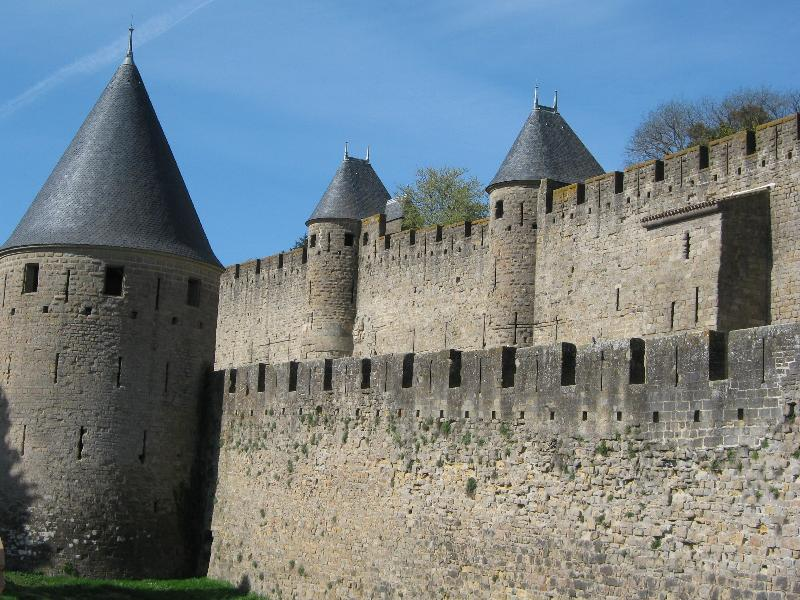
\includegraphics[width=0.95\textwidth]{assets/homography/castle_left}
    \end{minipage}%
    \hfill
    \begin{minipage}{.5\textwidth}
        \centering
    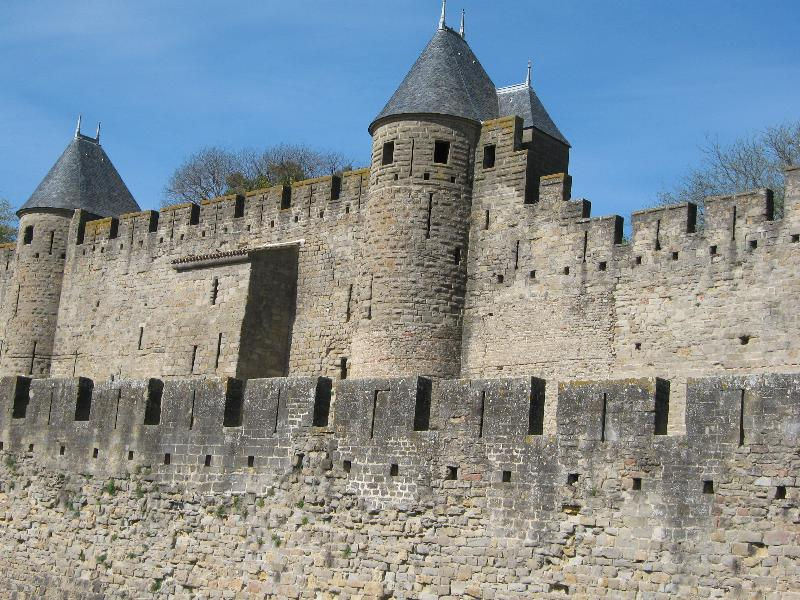
\includegraphics[width=0.95\textwidth]{assets/homography/castle_right}
    \end{minipage}
    \caption{The two input images.}
    \label{fig:castleimages}
\end{figure}

\begin{figure}[H]
    \centering
    \captionsetup{justification=centering}
    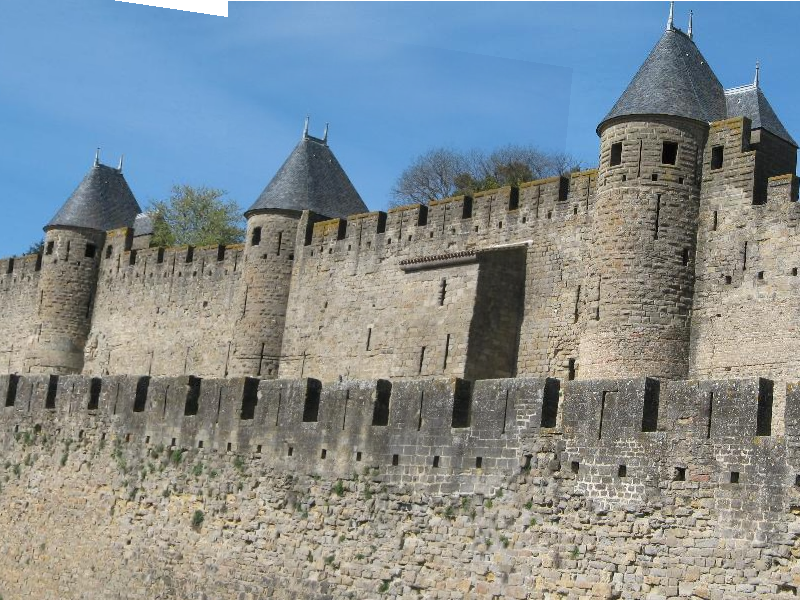
\includegraphics[width=0.475\textwidth]{assets/homography/castle_panorama}
    \caption{The stitched version of the images of figure~\ref{fig:castleimages} using paper~\citep{homography}.}
    \label{fig:panoramacastle}
\end{figure}

The homography matrix for the above stitching follows (\textit{QH.1}).

\[H=\left[
\begin{array}{c c c}
    1.16 & -0.11 & -525.59\\
    0.17 & 1.12 & -61.82\\
    2.18\times 10^{-4} & -2.89\times 10^{-5} & 1
\end{array}
\right]\]

As mentioned before, null values for $h_7$ and $h_8$ imply no change of perspective between the two images.
Here, $h_7$ and $h_8$ and are both very close to 0 which means that practically no perspective change occurred between
the two pictures of figure~\ref{fig:castleimages}, which seems plausible.

Comparatively, $h_3$ and $h_6$ are very large.
This is also plausible because they represent an overall translation in pixels (since $w'\approx 1$) and the images
are $800\times 600$.

The tool outputs not only the final panorama but also \textit{input images} and \textit{registered images}.

The input images 1 and 2 are simply the input images.
The registered images 1 and 2 are the two images that make up the final panorama.
That is, registered image 2 is simply the input image 2 but cropped (because the final panorama is of limited size
in this particular demo) and registered image 1 is the input image 1 but after the homography (and cropped as well).
This is because the authors decided to fix the second image and to warp the first one onto it: only the first image
is modified to build the panorama (\textit{QH.2}).

Taking the average of these two registered images pixel-wise gives the output panorama.

\begin{figure}[ht]
    \centering
    \captionsetup{justification=centering}
    \begin{minipage}{.5\textwidth}
        \centering
    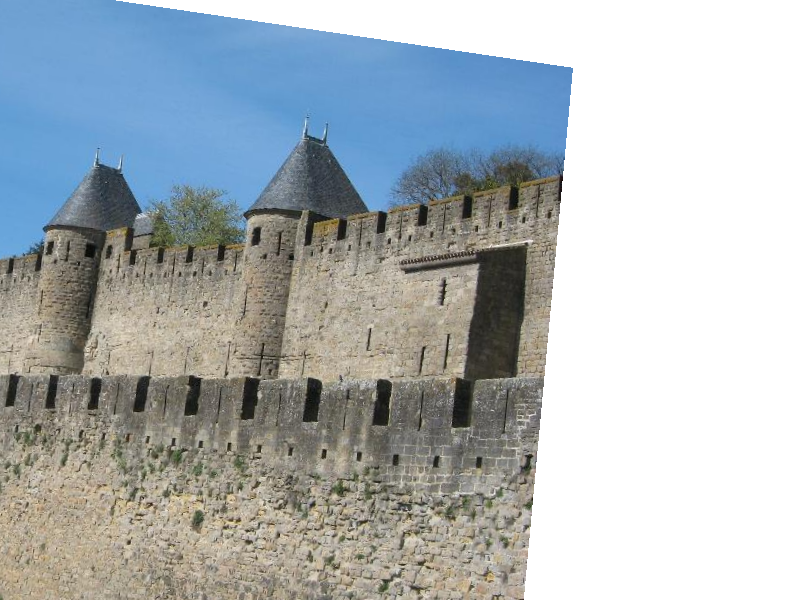
\includegraphics[width=0.95\textwidth]{assets/homography/reg_left}
    \end{minipage}%
    \hfill
    \begin{minipage}{.5\textwidth}
        \centering
    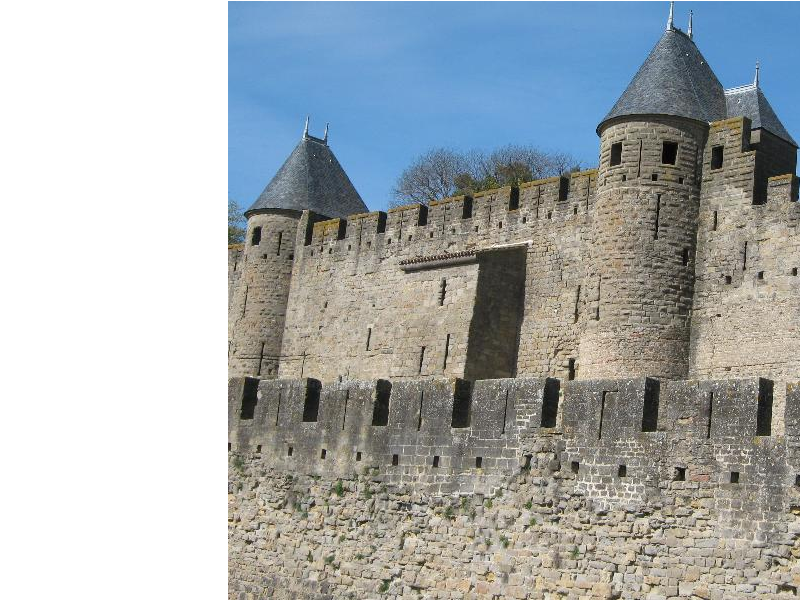
\includegraphics[width=0.95\textwidth]{assets/homography/reg_right}
    \end{minipage}
    \caption{The two \textit{registered} images.}
    \label{fig:regimages}
\end{figure}

The method used by the authors of~\citep{homography} is a modified RANSAC called ORSA (see figure~\ref{fig:orsa}).
They pick some set of points and compute the homography that best fits the points
(with the code of figure~\ref{fig:homographyfit}, \textit{QH.3}).

\begin{figure}[H]
    \centering
    \lstinputlisting[label={lst:orsa}]{assets/homography/orsa}
    \caption{(Simplified) code from~\citep{homography} that implements ORSA, their special RANSAC\@.}
    \label{fig:orsa}
\end{figure}

\begin{figure}[H]
    \centering
    \lstinputlisting[label={lst:homographyfit}]{assets/homography/homography_fit}
    \caption{(Simplified) code from~\citep{homography} to solve the system $Ah=0$.}
    \label{fig:homographyfit}
\end{figure}

For a specific set of $n$ points, they compute the homography and then the (ordered) vector of residues $(\epsilon_i)_i$
with $\epsilon_i = \left\|HP_i-P'_i\right\|_2$ where $P_i$ is the point in the left image and $P'_i$ the
corresponding point in the right image.
Using this vector of residues, they estimate the number of inliers using the $NFA$ (Number of False Alarms) which is a
measure of how likely it is to have these results if the number of inliers is $k$.
\[NFA=(n-4)\binom{n}{k}\binom{k}{4}\left(\epsilon_k^2\frac{\pi}{w'h'}\right)^{k-4}\]
The value of $k$ that minimizes this formula gives the number of inliers for the selected subset of points.

The $NFA$ (with optimized number of inliers $k$) also gives the measure of quality of $H$.
Hence, at each step, the homography with the smallest $NFA$ is kept (\textit{QH.4}).

Using this technique, we were able to stitch together four images into a larger panorama
(figure~\ref{fig:homography_img_1_2_3_4}, \textit{QH.5}).

\begin{figure}[ht]
    \centering
    \captionsetup{justification=centering}
    \begin{minipage}{.25\textwidth}
        \centering
    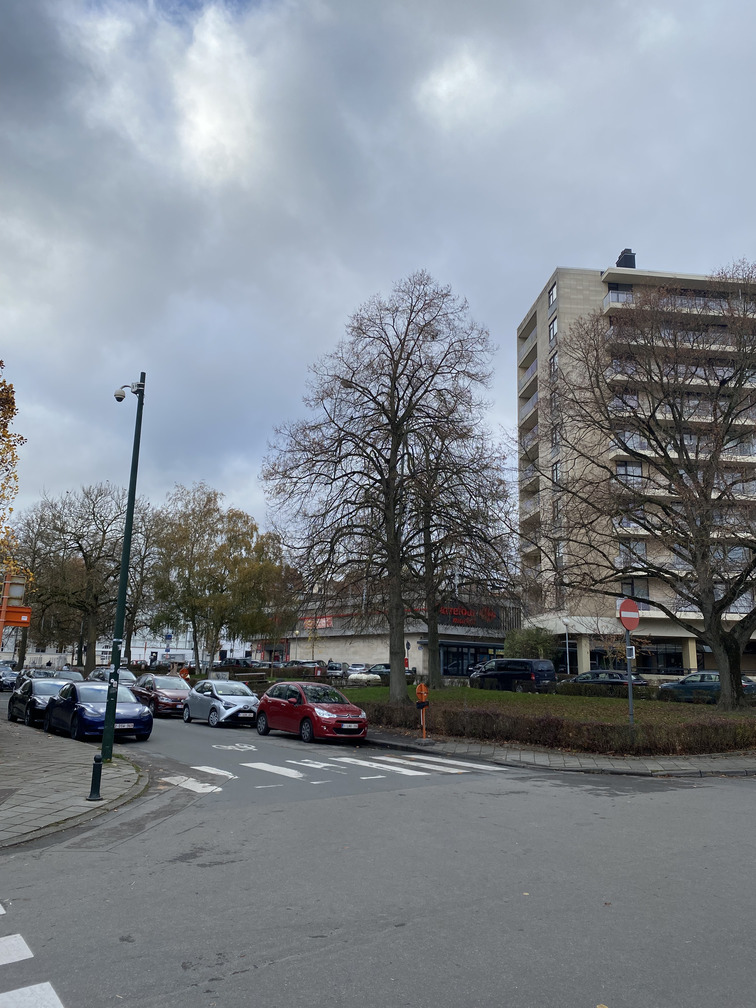
\includegraphics[width=0.95\textwidth]{assets/homography/img_1}
    \end{minipage}%
    \hfill
    \begin{minipage}{.25\textwidth}
        \centering
    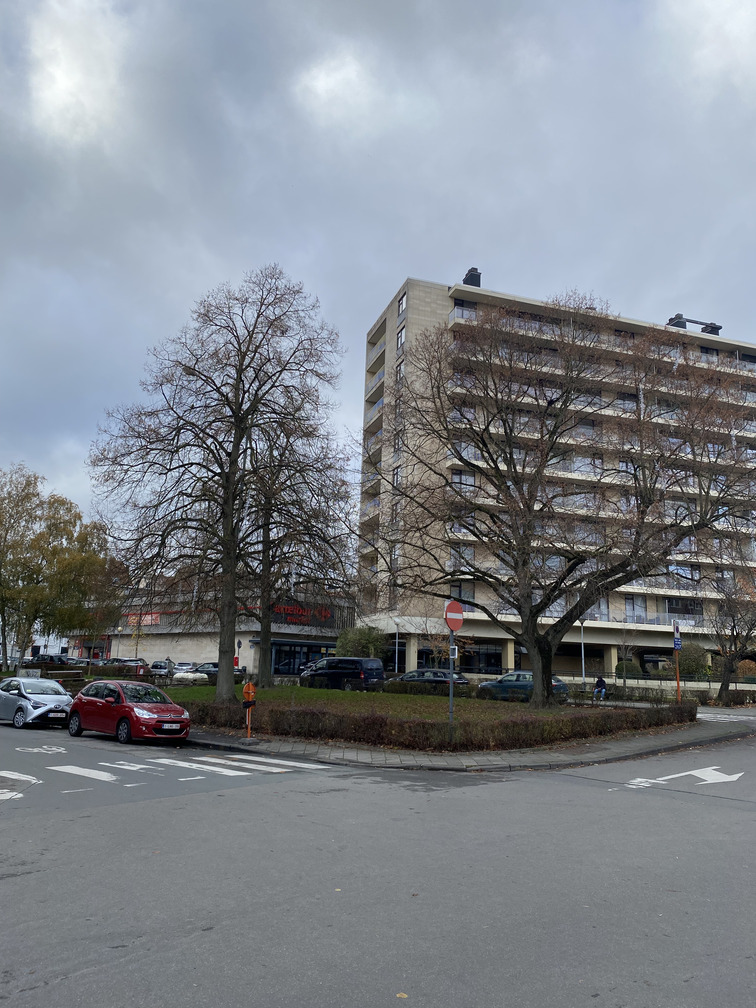
\includegraphics[width=0.95\textwidth]{assets/homography/img_2}
    \end{minipage}%
    \begin{minipage}{.25\textwidth}
        \centering
    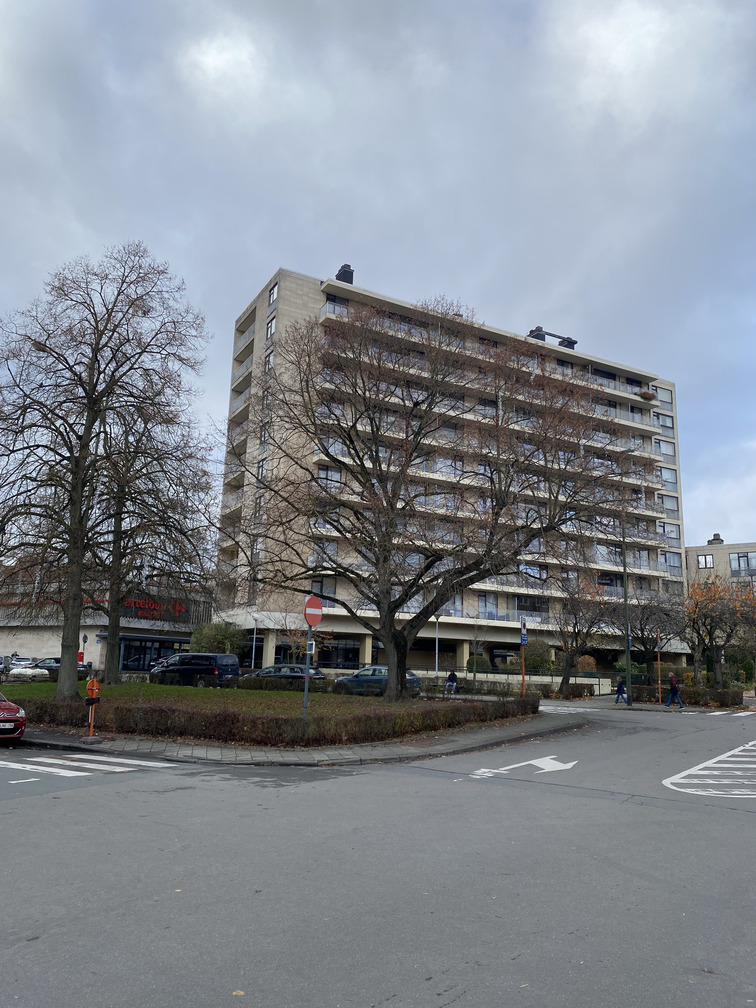
\includegraphics[width=0.95\textwidth]{assets/homography/img_3}
    \end{minipage}%
    \hfill
    \begin{minipage}{.25\textwidth}
        \centering
    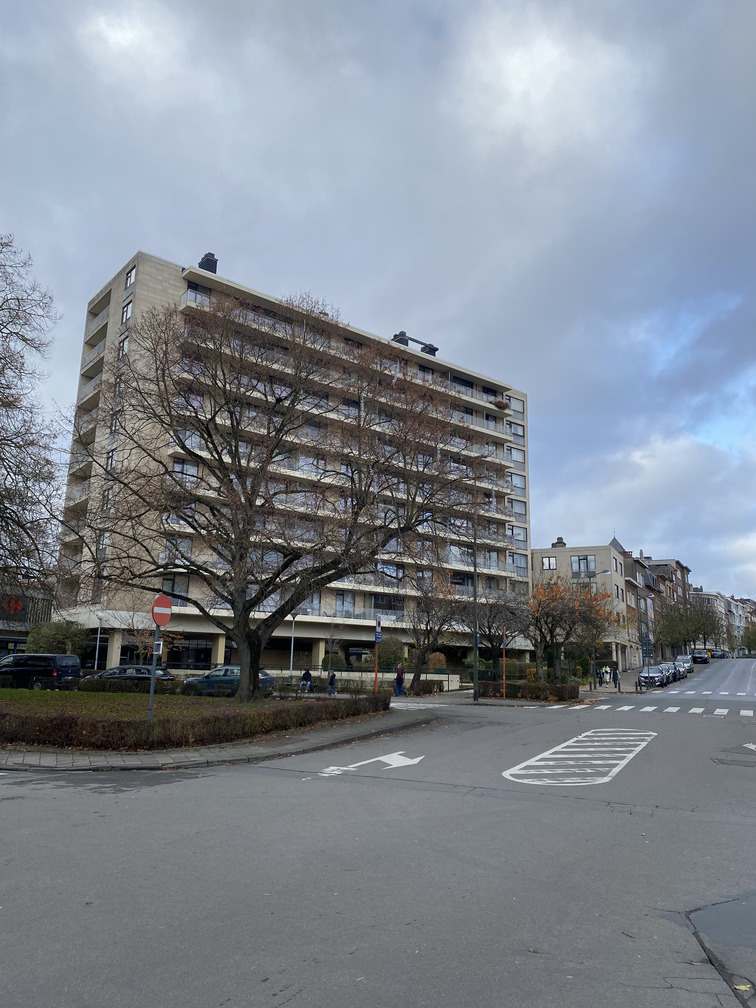
\includegraphics[width=0.95\textwidth]{assets/homography/img_4}
    \end{minipage}
    \caption{All images to be stitched.}
    \label{fig:homography_img_1_2_3_4}
\end{figure}

Using the online tool provided with the IPOL paper~\citep{homography}, we were able to find the homography matrices to
first stitch images 1 and 2, then images 3 and 4 and finally the two already stitched images into a full panorama.
We had to extract the homography matrices and perform the homography ourselves because the online tool crops the
resulting images to fit in the same frame as the input images.

\begin{figure}[ht]
    \centering
    \captionsetup{justification=centering}
    \begin{minipage}{.33\textwidth}
        \centering
    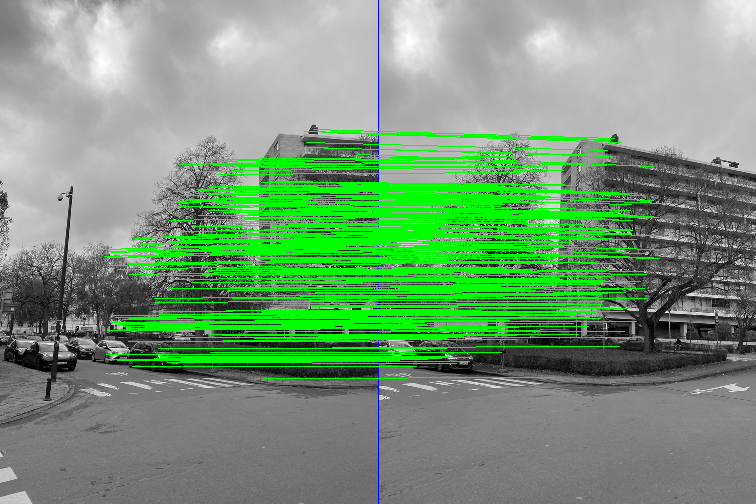
\includegraphics[width=0.95\textwidth]{assets/homography/img_12_inliers}
    \end{minipage}%
    \hfill
    \begin{minipage}{.33\textwidth}
        \centering
    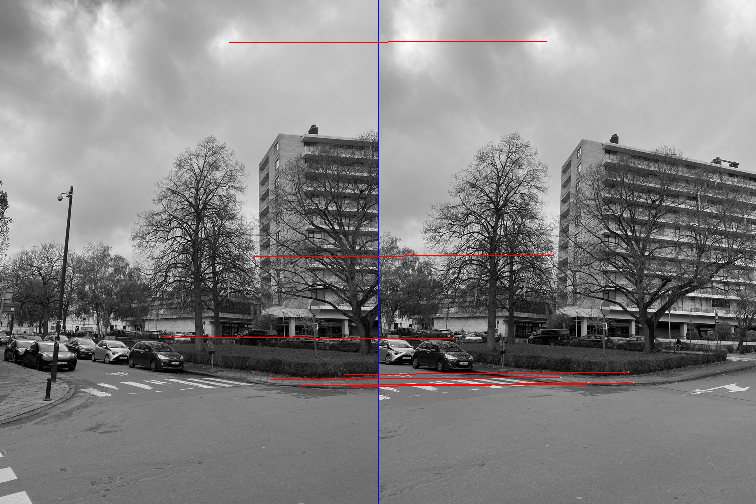
\includegraphics[width=0.95\textwidth]{assets/homography/img_12_outliers}
    \end{minipage}%
    \begin{minipage}{.33\textwidth}
        \centering
    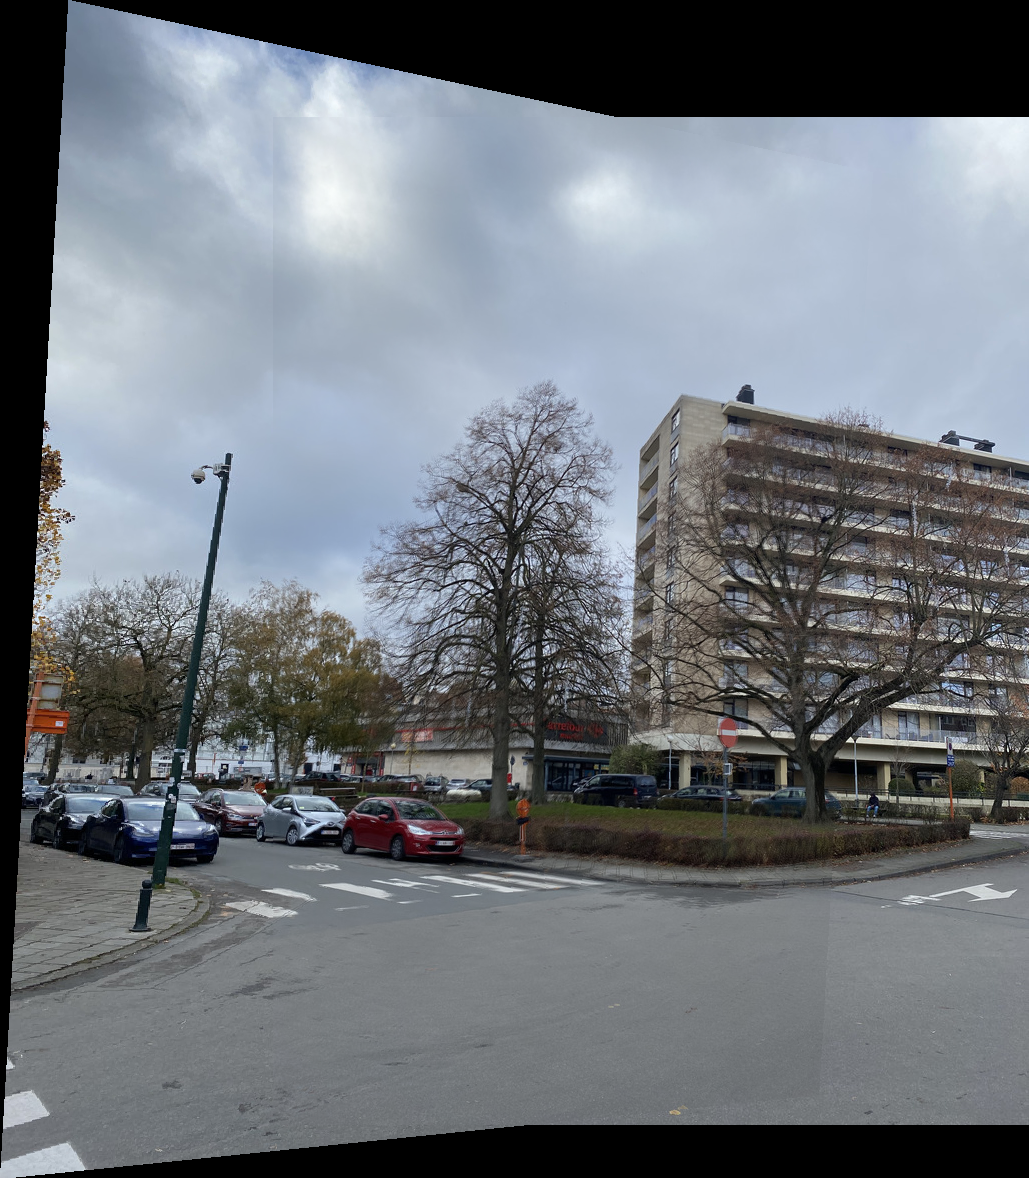
\includegraphics[width=0.95\textwidth]{assets/homography/img_12}
    \end{minipage}
    \caption{Stitched images 1 and 2 alongside the detected inliers and outliers.}
    \label{fig:homography_img_12}
\end{figure}

\begin{figure}[ht]
    \centering
    \captionsetup{justification=centering}
    \begin{minipage}{.33\textwidth}
        \centering
    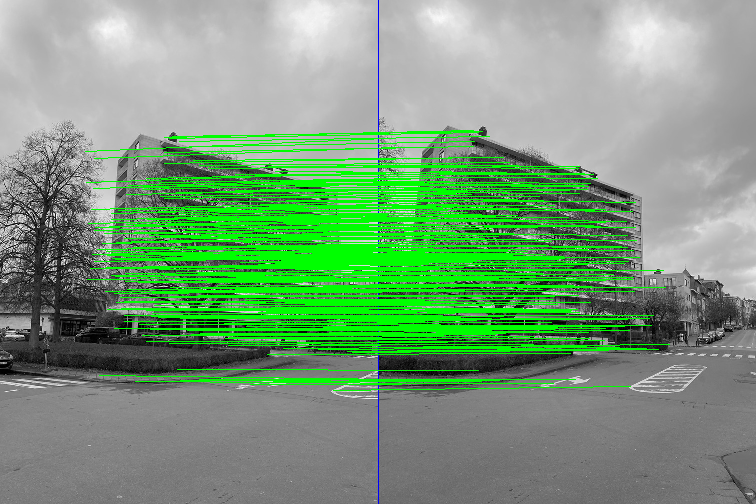
\includegraphics[width=0.95\textwidth]{assets/homography/img_34_inliers}
    \end{minipage}%
    \hfill
    \begin{minipage}{.33\textwidth}
        \centering
    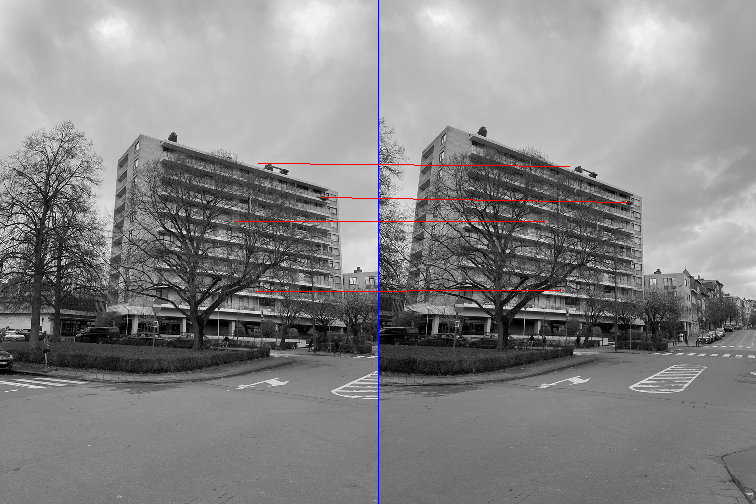
\includegraphics[width=0.95\textwidth]{assets/homography/img_34_outliers}
    \end{minipage}%
    \begin{minipage}{.33\textwidth}
        \centering
    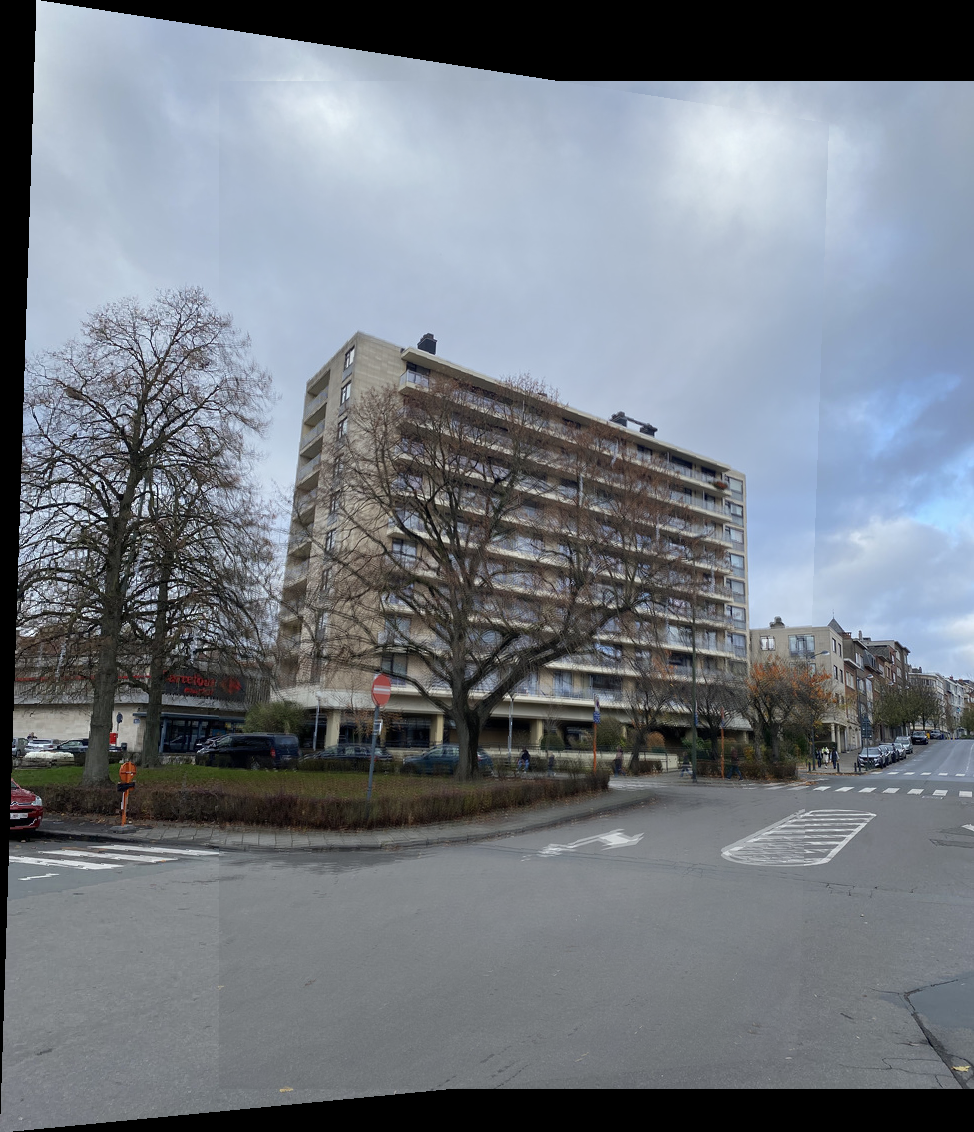
\includegraphics[width=0.95\textwidth]{assets/homography/img_34}
    \end{minipage}
    \caption{Stitched images 3 and 4 alongside the detected inliers and outliers.}
    \label{fig:homography_img_34}
\end{figure}

In both figures~\ref{fig:homography_img_12} and~\ref{fig:homography_img_34}, we can observe that the stitching is
blurry on points that are close to the camera (the roads).
This is because homography for stitching only works with flat scenes (or far away scenes).

\begin{figure}[ht]
    \centering
    \captionsetup{justification=centering}
    \begin{minipage}{.5\textwidth}
        \centering
    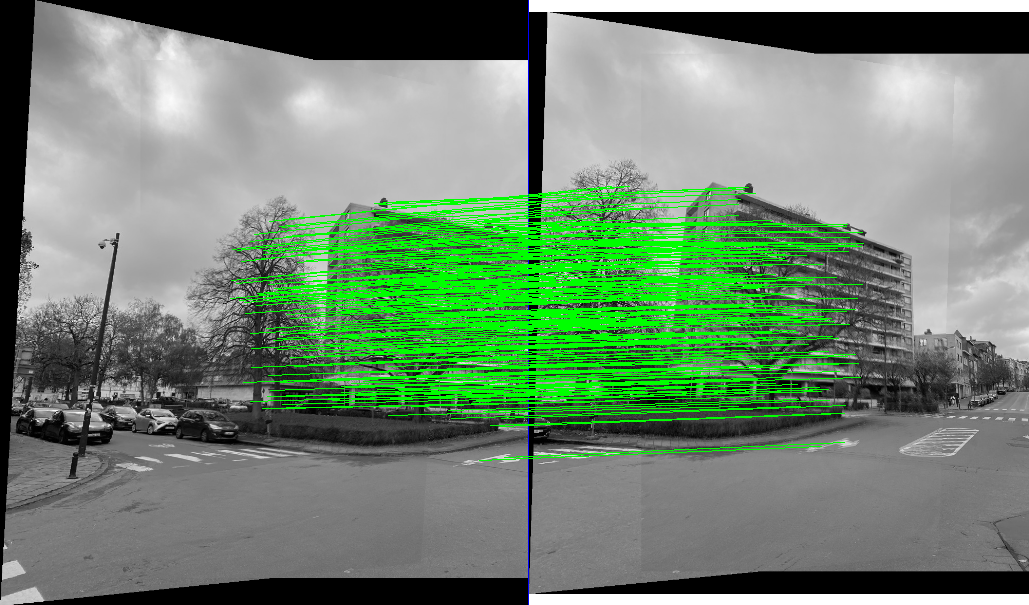
\includegraphics[width=0.95\textwidth]{assets/homography/img_1234_inliers}
    \end{minipage}%
    \hfill
    \begin{minipage}{.5\textwidth}
        \centering
    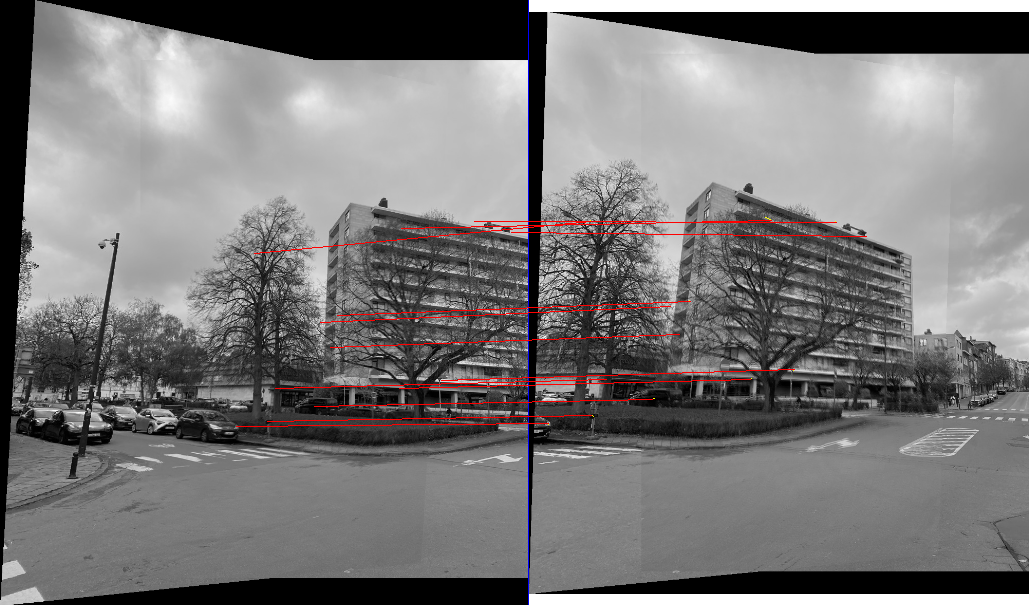
\includegraphics[width=0.95\textwidth]{assets/homography/img_1234_outliers}
    \end{minipage}
    \label{fig:homography_inliers_img_1234}
\end{figure}

\begin{figure}[ht]
    \centering
    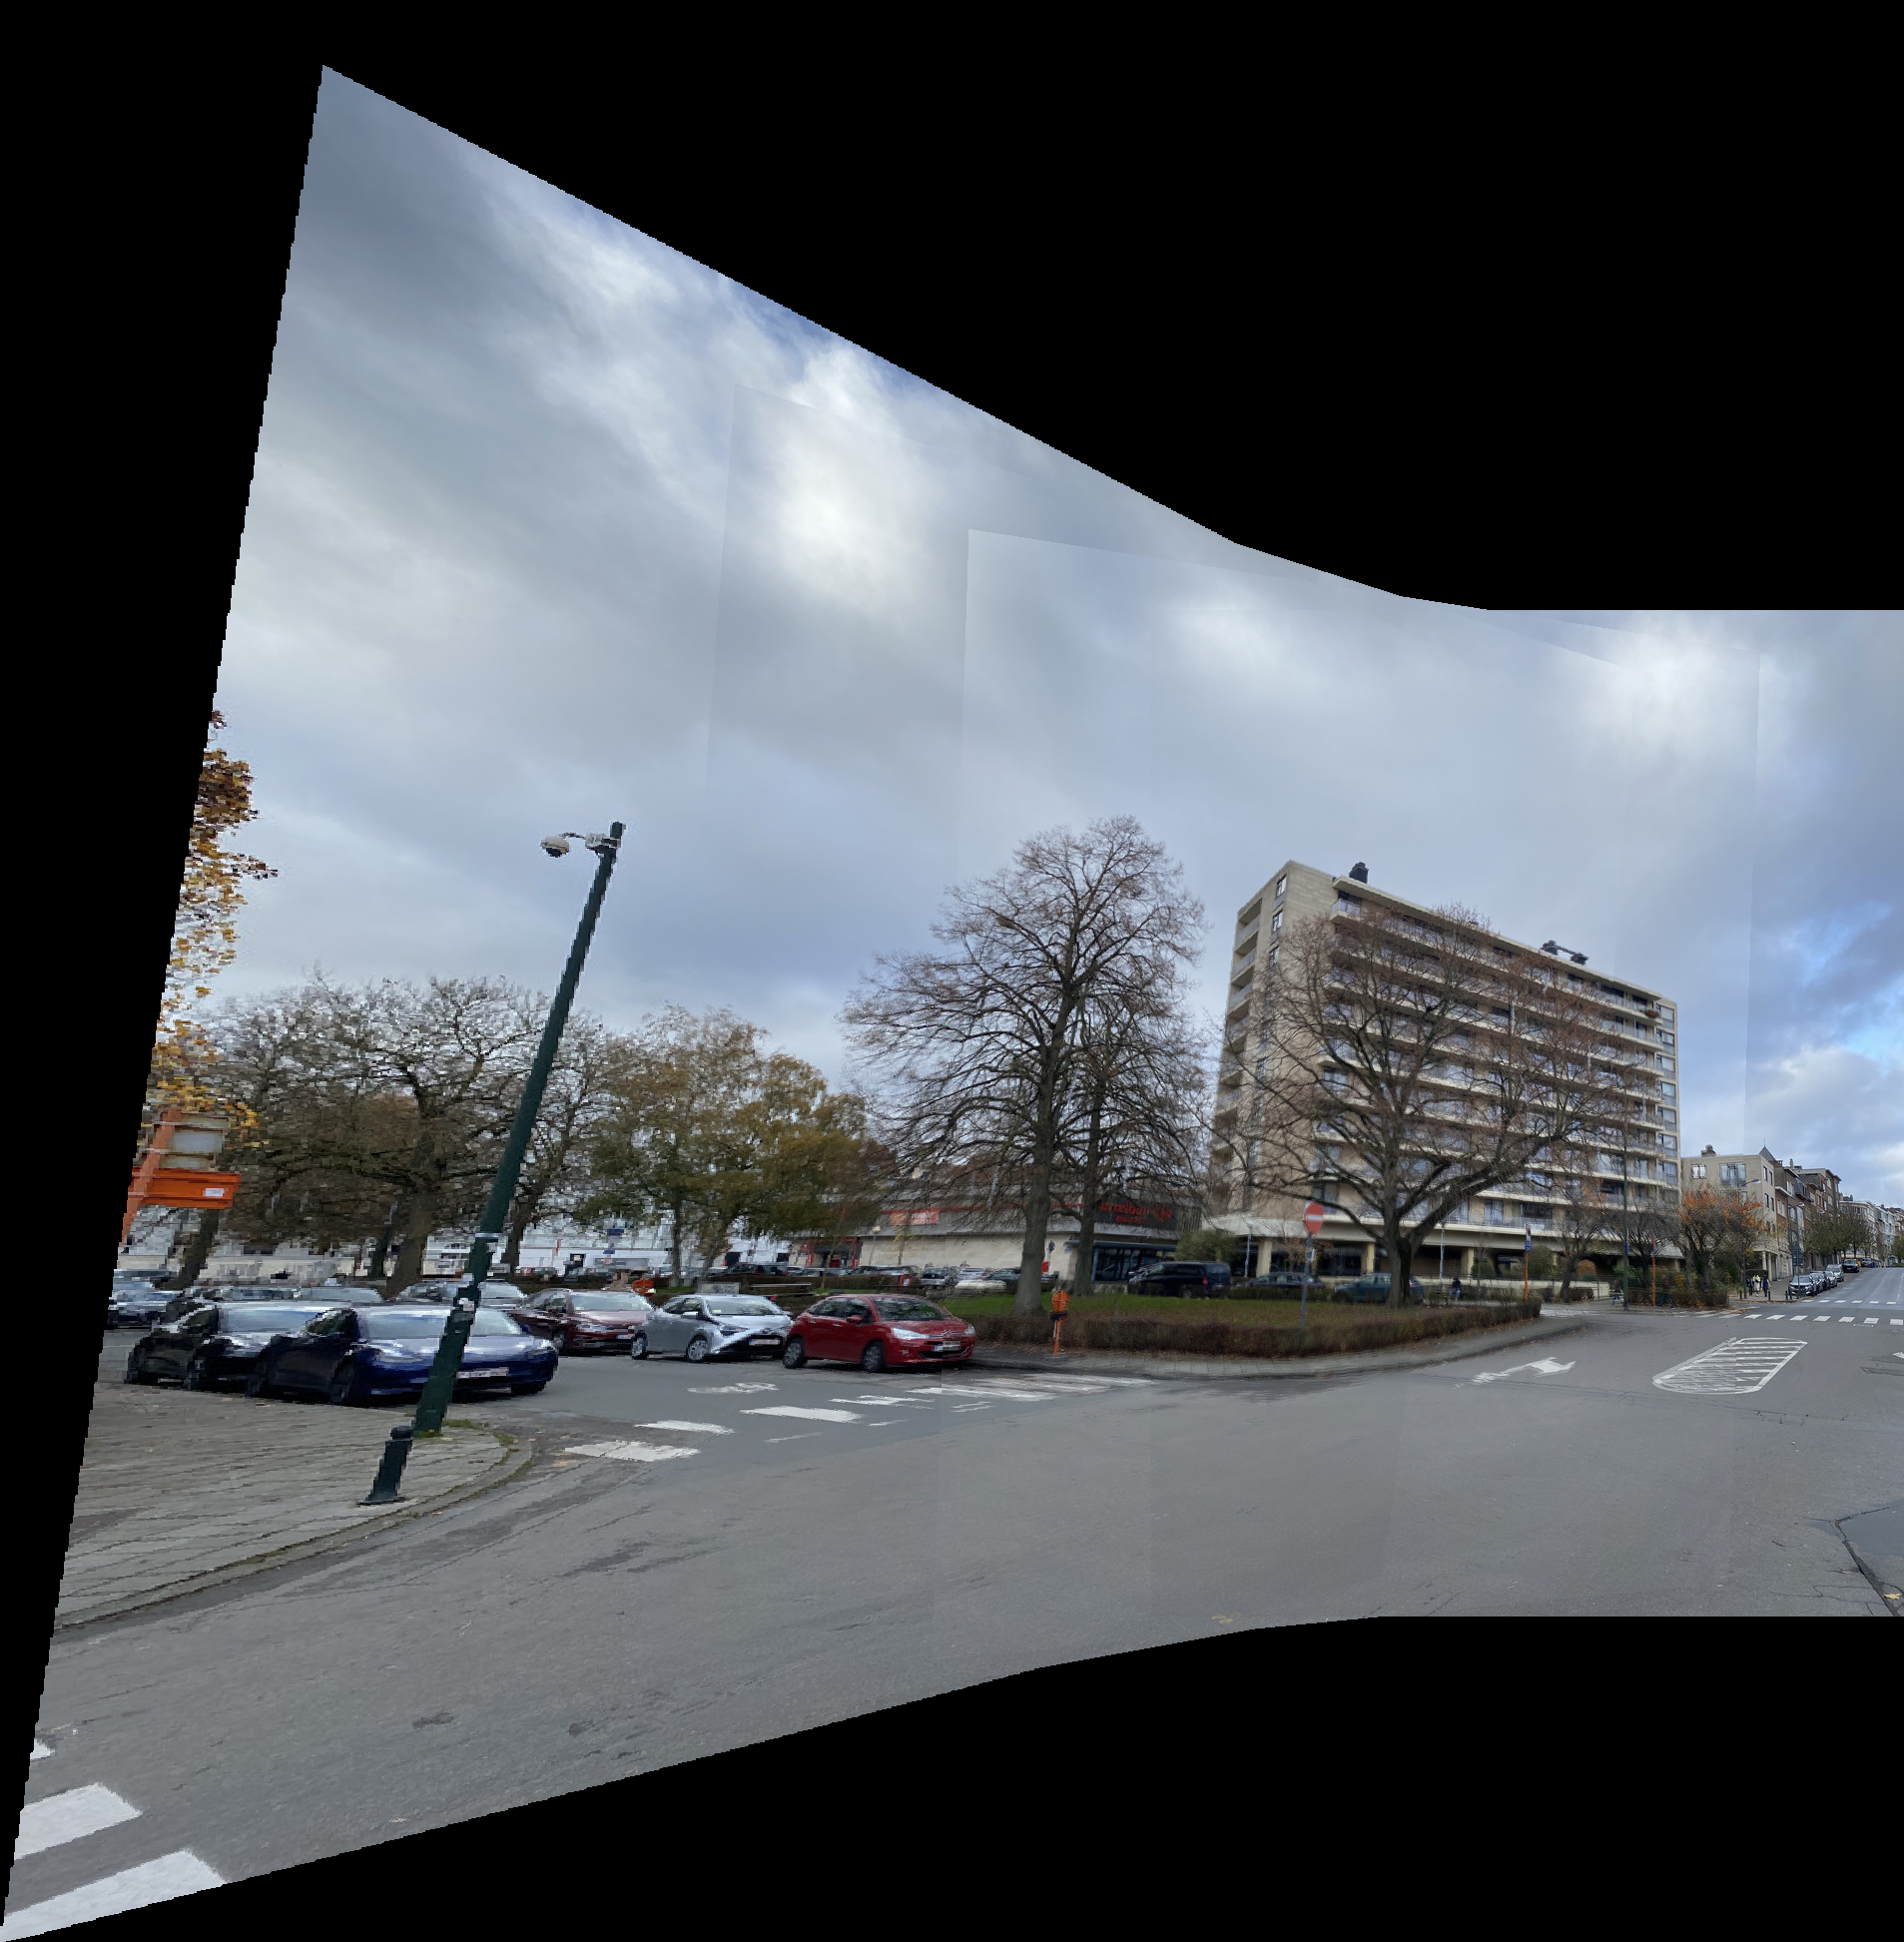
\includegraphics[width=0.65\textwidth]{assets/homography/img_1234}
    \caption{The final stitched panorama.}
    \label{fig:homography_img_1234}
\end{figure}

As we can observe in figure~\ref{fig:homography_img_1234}, the leftmost image was repeatedly distorted and became less
detailed.

For the sake of completeness, we provide the homography matrices found for each stitching.

\begin{gather*}
    \begin{array}{c c}
      H_{12}=\left[
\begin{array}{c c c}
    1.284 & -0.068 & -204.83\\
    0.248 & 1.17 & -116.55\\
    0.000367 & 0.000000189 & 1
\end{array}
\right] &
      H_{34}=\left[
\begin{array}{c c c}
    1.222 & -0.037 & -182.31\\
    0.175 & 1.127 & -81.10\\
    0.000285 & 0.00000303 & 1
\end{array}
\right]\end{array}\\
    H_{1234}=\left[
\begin{array}{c c c}
    2.037 & -0.123 & -782.54\\
    0.583 & 1.644 & -530.255\\
    0.000821 & -0.00000562 & 1
\end{array}
\right]
\end{gather*}

    \subsection{Rectification}\label{subsec:rectification}

The rectification of two images is a process that finds two homographies $H_1$ and $H_2$ such that the two
homographied images have horizontal epipolar lines (or alternatively that the pixels of one image are all found at the
same $y$-level in the other image).

The first step of the algorithm is to run SIFT and match corresponding pairs of points.
ORSA (or RANSAC) is used to remove outliers (exactly as in the previous section) and find the fundamental matrix $F$.

The fundamental equation of epipolar geometry related how two corresponding points in two images must relate,
where $P_1$ and $P_2$ are the image coordinates of the two corresponding points (in homogeneous coordinates) and
$F$ is the fundamental matrix.
\begin{equation}\label{eq:fundamentalequationepipolargeometry}
    P_2^t F P_1=0
\end{equation}
In particular, equation~\eqref{eq:fundamentalequationepipolargeometry} states that if we know where a point is within
an image, the corresponding point in the other image will lie on a line.

If the images are rectified,
\[F=[e_1]_{\times}=\left[
\begin{array}{c c c}
    0 & 0 & 0\\
    0 & 0 & -1\\
    0 & 1 & 0
\end{array}\right]\]

This means that finding two homographies $H_R$ and $H_L$ such that:
\[F= H_R^t [e_1]_{\times} H_L\]
Is enough to rectify the two images since, by equation~\eqref{eq:fundamentalequationepipolargeometry}:
\[(H_R P_2)^t [e_1]_{\times} (H_L P_1) =0\]

The idea of the authors of~\citep{rectification} is to find rotations $R_R$ and $R_L$ that will rectify the images.
Rotating the camera with a rotation matrix $R$ is equivalent to the following homography $H$ (with $K$ the intrinsics
of the camera).
\[H=K R K^{-1}\]
Note that $K$ is not known in advance: $f$ is found at the same time as $R_R$ and $R_L$, and the principal point is
assumed to be at the center of both images.

Thus, the authors want to find $R_R$, $R_L$ and $f$ such that (note that $K^t [e_1]_{\times} K=f^2[e_1]_{\times})$:
\begin{align*}
    E(P_1,P_2,R_R,R_L,f)&=(K R_R K^{-1} P_2)[e_1]_{\times} (K R_L K^{-1} P_2)=P_2^t K^{-t} R_R^t K^t [e_1]_{\times} K R_L K^{-1} P_2\\
    &=P_2^t K^{-t} R_R^t f^2[e_1]_{\times} R_L K^{-1} P_2=0
\end{align*}

This can be reparametrized with $s=(\theta_{Ry},\theta_{Rz},\theta_{Lx},\theta_{Ly},\theta_{Lz},g)$ such that:
\[R_R=R_z(\theta_{Rz})R_y(\theta_{Ry})\hspace*{2em}R_L=R_z(\theta_{Lz})R_y(\theta_{Ly})R_x(\theta_{Lx})
\hspace*{2em} f=3^g (w+h)\]

Instead of minimizing the above error (which has no geometric interpretation but arises from algebra only), they
minimize the Sampson error:
\begin{equation}\label{eq:errorrectification}
    E_s(P_1,P_2)^2=E^t(JJ^t)^{-1}E
\end{equation}
Where $J$ is the jacobian of $E$ (in particular, computing $J$ requires the computation of
$\frac{\partial F}{\partial \theta_{Ry}},\frac{\partial F}{\partial \theta_{Rz}},\ldots$).

Using the continuous optimization algorithm of Levenberg-Marquardt, it is possible to find the best values for
$s=(\theta_{Ry},\theta_{Rz},\theta_{Lx},\theta_{Ly},\theta_{Lz},g)$ that minimize the sum of $E_s(P_1,P_2)^2$ for all
pairs of inlier points (\textit{QR.5}).

Figure~\ref{fig:rectification_base_images} shows two images of the same scene that we will rectify using the online
IPOL demo~\citep{rectification}.

\begin{figure}[ht]
    \centering
    \captionsetup{justification=centering}
    \begin{minipage}{.5\textwidth}
        \centering
    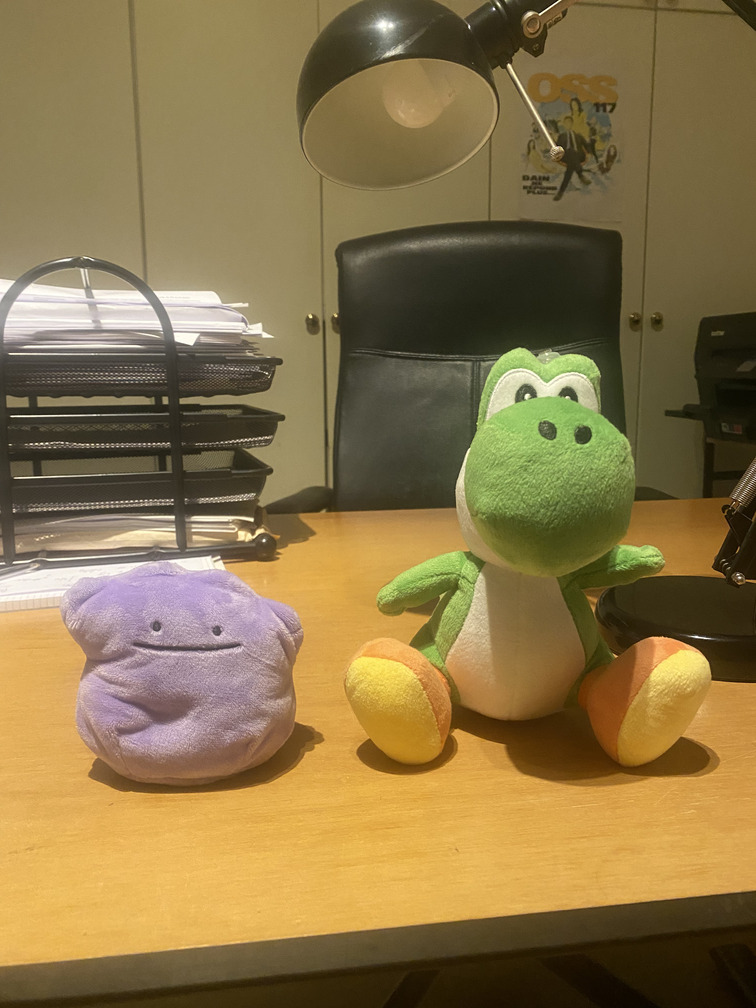
\includegraphics[width=0.6\textwidth]{assets/rectification/img_left}
    \end{minipage}%
    \hfill
    \begin{minipage}{.5\textwidth}
        \centering
    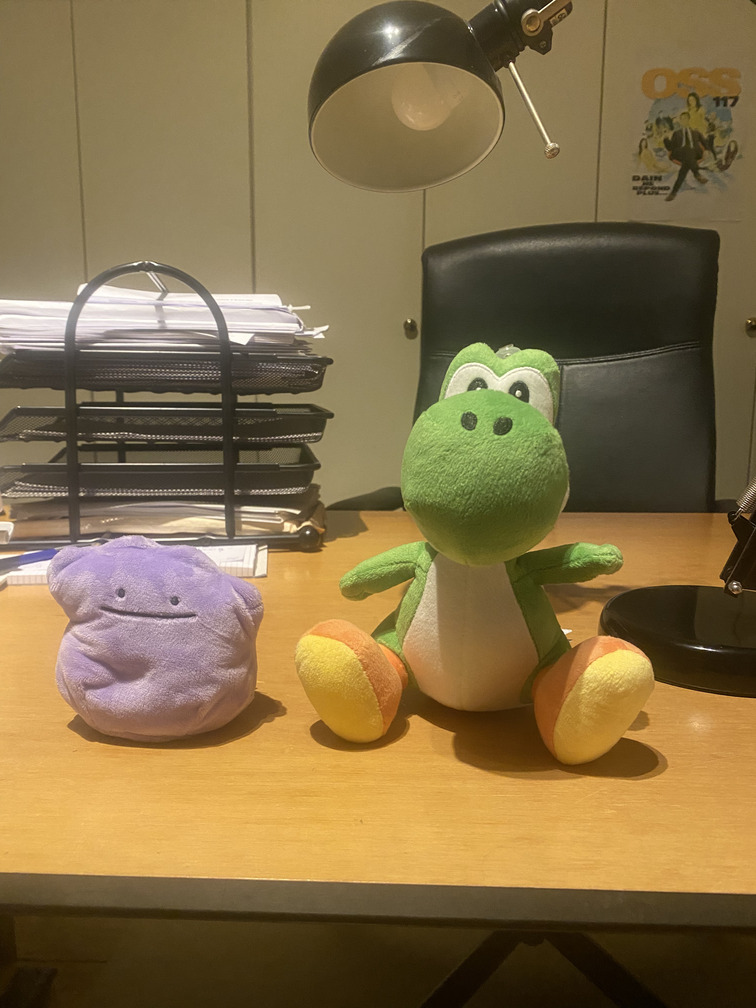
\includegraphics[width=0.6\textwidth]{assets/rectification/img_right}
    \end{minipage}
    \caption{The two original images.}
    \label{fig:rectification_base_images}
\end{figure}

The rectified pair is given in figure~\ref{fig:rectified_images} (\textit{QR.1}, a \texttt{gif} version is provided
alongside this report).

\begin{figure}[ht]
    \centering
    \captionsetup{justification=centering}
    \begin{minipage}{.5\textwidth}
        \centering
    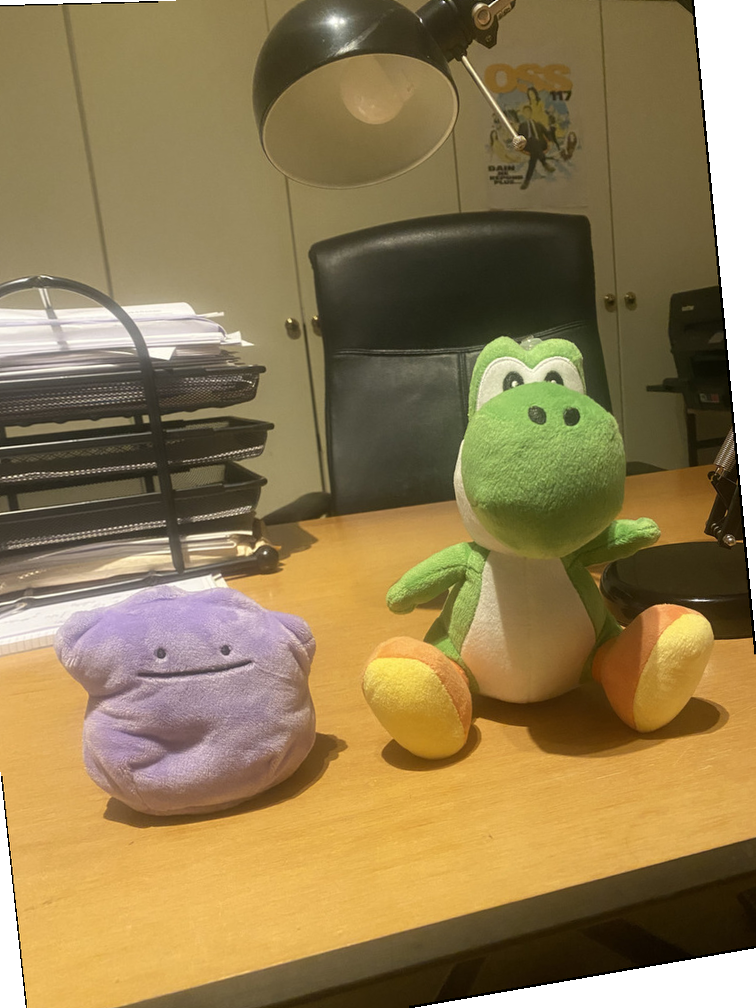
\includegraphics[width=0.6\textwidth]{assets/rectification/img_left_rect}
    \end{minipage}%
    \hfill
    \begin{minipage}{.5\textwidth}
        \centering
    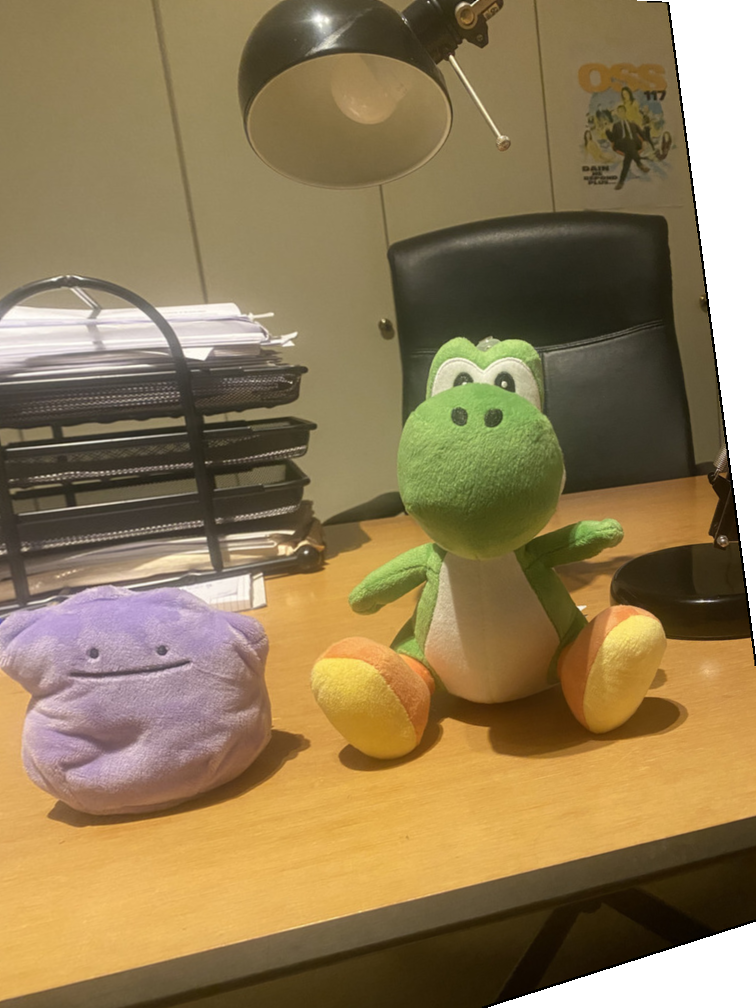
\includegraphics[width=0.6\textwidth]{assets/rectification/img_right_rect}
    \end{minipage}
    \caption{The two rectified images.}
    \label{fig:rectified_images}
\end{figure}

As mentioned before, the tool finds two homographies and applies them to the input images to find the rectified pair.
We give hereunder the homography for the right image.
\[H_R=\left[
\begin{array}{c c c}
    1.156 & 0.157 & -150.34\\
    0.0374 & 1.0078 & -26.91\\
    0.00035 & 0.0000349 & 0.81749
\end{array}\right]\]
We can verify that this homography indeed corresponds to the rectification of the right image by applying
it (\textit{QR.2}):
\begin{figure}[ht]
    \centering
    \captionsetup{justification=centering}
    \begin{minipage}{.5\textwidth}
        \centering
    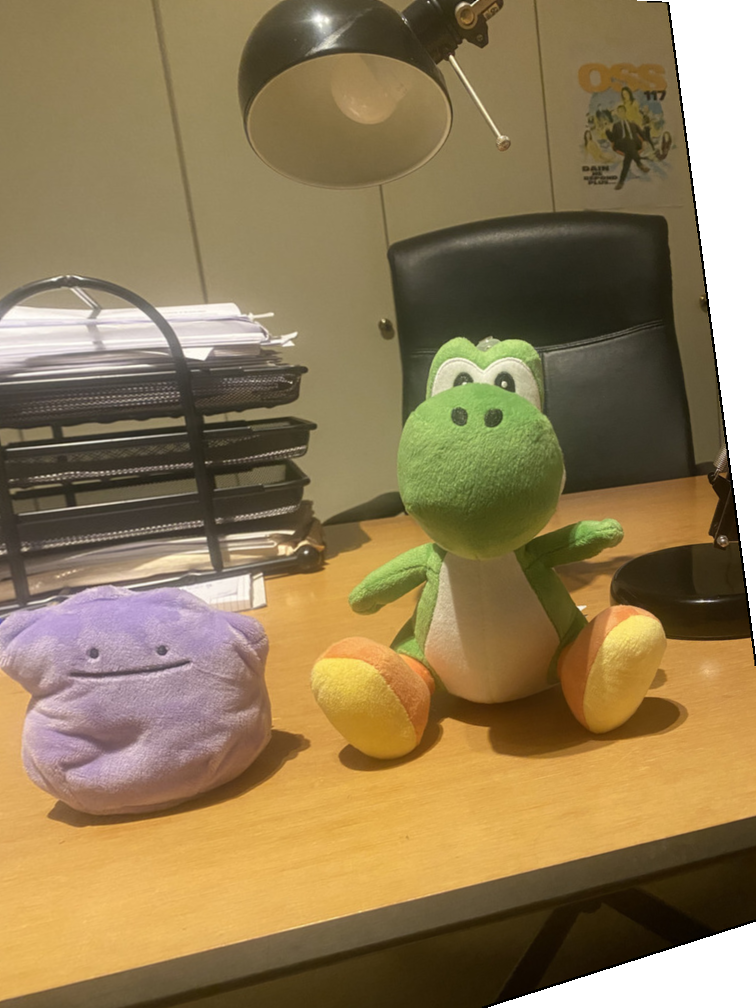
\includegraphics[width=0.6\textwidth]{assets/rectification/img_right_rect}
    \end{minipage}%
    \hfill
    \begin{minipage}{.5\textwidth}
        \centering
    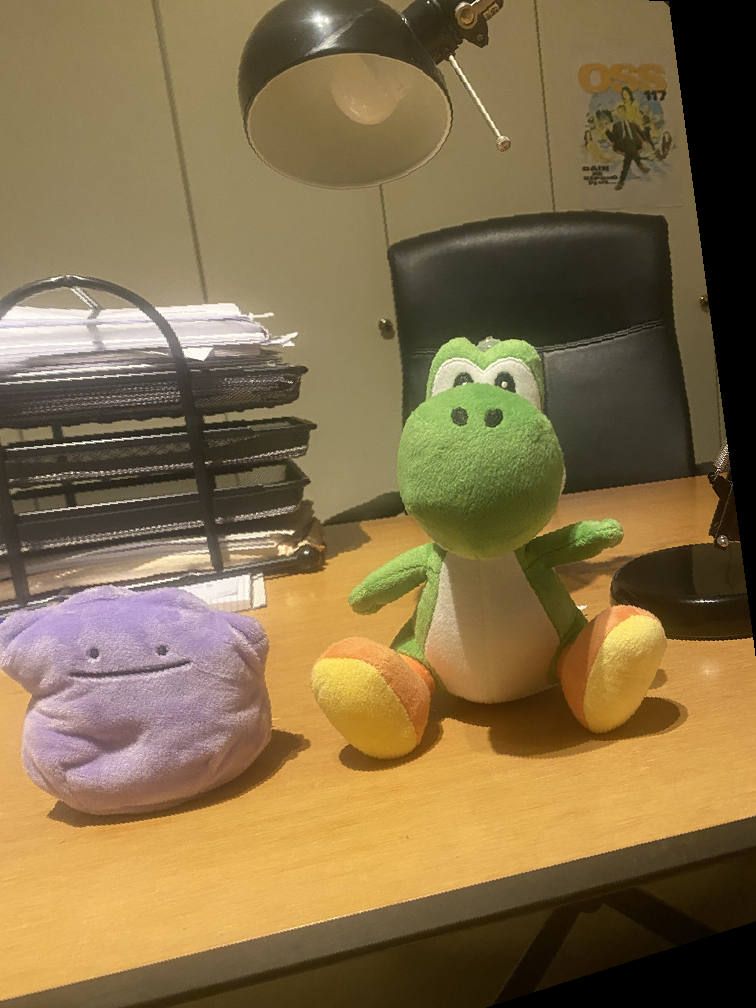
\includegraphics[width=0.6\textwidth]{assets/rectification/homographied_right_img}
    \end{minipage}
    \caption{The right output image (left) and the right input image homographied by $H_R$ (right).}
    \label{fig:righthomographiedimage}
\end{figure}

We will draw the epipolar line corresponding to the right armpit of Yoshi in the left image.
The right armpit of Yoshi lies at the point $(459,577)$, which means that $P_1=\left[\begin{array}{c c c}
                   459 & 577 &1\end{array}\right]^t$.
The online tool estimated $F$ for us.

\[F=\left[
\begin{array}{c c c}
    -1.41539e-08 & 2.82758e-07 & -1.6399e-05\\
    -8.97881e-08 & 7.82147e-09 & -0.0009103\\
    -3.28468e-05 & 0.000803705 & 0.0285408
\end{array}
\right]\]

Since we know $P_1$ and $F$, we can compute the epipolar line.
If $FP_1=\left[\begin{array}{c c c}
                   a & b & c
\end{array}\right]^t $, then the equation of the epipolar line is
(by equation~\eqref{eq:fundamentalequationepipolargeometry}):
\[y=\frac{-ax-c}{b}\]
In figure~\ref{fig:yoshi_epipolar}, we show this epipolar line, and we can observe that indeed, the right armpit of Yoshi
lies on the line (\textit{QR.3}).

\begin{figure}[ht]
    \centering
    \captionsetup{justification=centering}
    \begin{minipage}{.5\textwidth}
        \centering
    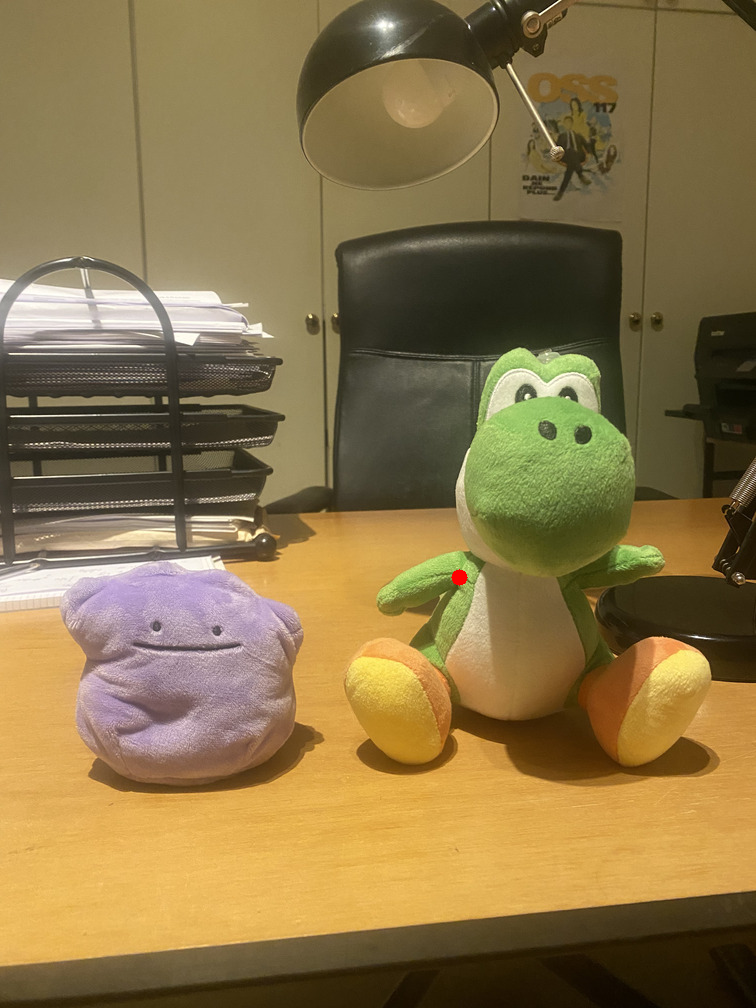
\includegraphics[width=0.7\textwidth]{assets/rectification/yoshi_epipolar_left}
    \end{minipage}%
    \hfill
    \begin{minipage}{.5\textwidth}
        \centering
    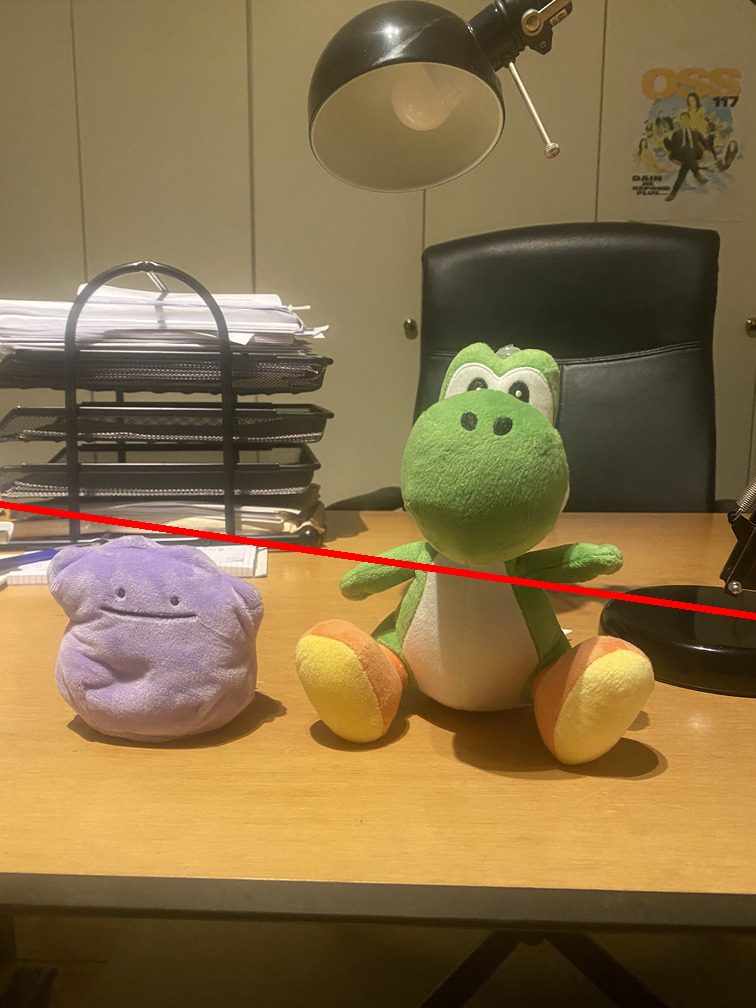
\includegraphics[width=0.7\textwidth]{assets/rectification/yoshi_epipolar_right}
    \end{minipage}
    \caption{The two original images but with the epipolar line (in the right image) corresponding to the point on the
    right armpit of Yoshi (in the left image).}
    \label{fig:yoshi_epipolar}
\end{figure}

The focal length was estimated by the online tool, and we are thus able to build the two intrinsics matrices (assuming
the principal point is in the center of the $756\times 1006$ pixels images).
Note that the $K_1$, $K_2$ matrices that the tool outputs are the intrinsics for the cameras of the homographied images.
\[K_L=\left[
\begin{array}{c c c}
    731.057 & 0 & 378\\
    0 & 731.057 & 504\\
    0 & 0 & 1
\end{array}\right]\hspace*{2em}
K_R=\left[
\begin{array}{c c c}
    731.057 & 0 & 378\\
    0 & 731.057 & 504\\
    0 & 0 & 1
\end{array}\right]\]

The essential matrix $E=RT_{[\times]}$ holds information about the translation and rotation between the two shots.
The fundamental matrix can be written as the following product (which thus holds both the intrinsics and
extrinsics)\footnote{There is a typo in the syllabus, it's written $F=K_R^t EK_L$ on page 31.}:
\begin{equation*}
    E=K_R^t FK_L
\end{equation*}
We would like to retrieve the rotation and translation information for the two shots.
Using Singular Value Decomposition (SVD), we can decompose $E$:
\[E=RT_{[\times]}=U\Sigma V^t\]
With all three matrices above, it is possible to retrive $R$ and $T_{[\times]}$ out of four different possibilities:
\begin{align*}
        T_{[\times]}&=U(\pm W)\Sigma U^t\\
        R&=U(\pm W)^{-1}V^t
\end{align*}

Where:
\[\pm W=\left[\begin{array}{c c c}
              0 & \pm 1 & 0\\
              \mp 1 & 0 & 0\\
              0 & 0 & 1
\end{array}\right]\]

We can apply this procedure on the two images of figure~\ref{fig:rectification_base_images}.
This gives four different possibities for $(R,t)$ with only one that is correct.
We extrinsics between the left and the right shot are (\textit{QR.4}):
\[t=\lambda\left[\begin{array}{c c c}
    0.572 & 0.0713 & -0.138
\end{array}\right]^t\hspace*{2em}R=\left[\begin{array}{c c c}
    0.987 & -0.0397 & 0.151 \\
    0.0392 & 0.999 & 0.00637 \\
    -0.151 & -0.000371 & 0.989
\end{array}\right]\]
We were able to isolate the correct pair $(R,t)$ because only one of the two possible $t$ had a positive $x$ component
and only one of the two possible $R$ did not make the camera look into the opposite direction (flipped the $z$ axis).

We can visualize these extrinsics using an online tool such as
\\\href{https://dugas.ch/transform_viewer/index.html}{https://dugas.ch/transform\_viewer/index.html}
(figure~\ref{fig:rect_twocameras}).

\begin{figure}[H]
    \centering
    \captionsetup{justification=centering}
    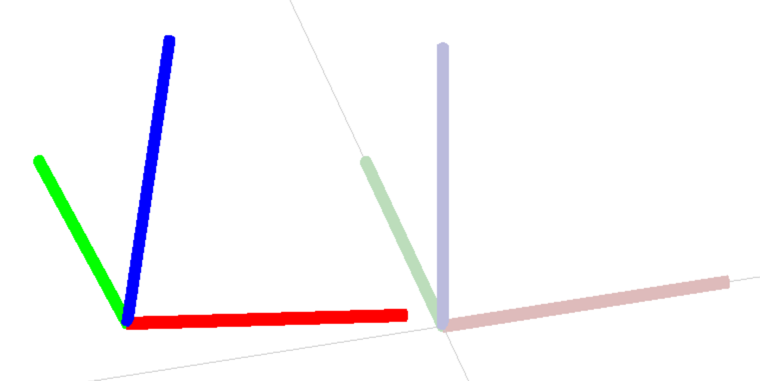
\includegraphics[width=0.4\textwidth]{assets/rectification/twocameras}
    \caption{The position in space of the two cameras according to the found extrinsics $R,t$.
    Note that the $x$-axis (red) is flipped and the $z$-axis (blue) is the depth axis.
    The dim origin represents the position of the left camera and the brighter one the right camera.}
    \label{fig:rect_twocameras}
\end{figure}

The issue is that the translation is only known up to scale.
To retrieve the size of the baseline, we can approximate the depth of some pixel and its disparity and then apply
the following equation to retrieve the baseline, where $Z$ is the depth (in $mm$), $B$ the baseline (in $mm$), $f$
the focal length (in $px$) and $d$ the disparity (in $px$):

\begin{equation}\label{eq:disparitydepth}
    Z=B\frac{f}{d}\Longleftrightarrow B=\frac{dZ}{f}
\end{equation}

We will consider the upmost point of Yoshi's two eyes.
The top pixel of Yoshi's right eye (the one on the left from the camera's point of view) is located at $(512,372)$ and
left eye is located at $(552,370)$.
We have $\Delta x'=552-512=40$ and $\Delta y'=372-370=2$.

We have seen in the lecture that the image point $(x',y')$ has the coordinates $(X,Y,Z)$ is 3D space, where:
\[x'=p_x+\frac{f_x X}{Z}\hspace*{2em} y'=p_y+\frac{f_y Y}{Z}\]
Here, $f_x=f_y=f$.
Rearranging the terms,
\[X=\frac{Z(x'-p_x)}{f}\hspace*{2em} Y=\frac{Z(y'-p_y)}{f}\]
We have that the difference in $X$ and $Y$ coordinates of the two considered points is:
\[\Delta X=X_1-X_2=\frac{Z(x'_1-p_x)}{f}-\frac{Z(x'_2-p_x)}{f}=\frac{Z\Delta x'}{f}\hspace*{2em} \Delta Y=\frac{Z\Delta y'}{f}\]
Note that we want to find the depth $Z$.
The real-life distance between the top of the two eyes is of approximately $D=19.3mm$.
This distance is equal to ($\Delta Z=0$ since we have picked points at the same depth):
\[D=\sqrt{\Delta X^2+\Delta Y^2+\Delta Z^2}=\sqrt{\Delta X^2+\Delta Y^2}\]
Combining everything, we have:
\[D=\sqrt{\left(\frac{Z\Delta x'}{f}\right)^2+\left(\frac{Z\Delta y'}{f}\right)^2}=\frac{Z}{f}\sqrt{(\Delta x')^2+(\Delta y')^2}\]
Finally, rearranging the terms:
\[Z=\frac{Df}{\sqrt{(\Delta x')^2+(\Delta y')^2}}\]
Plugging in $f=731.057$ (found by the only tool), $\Delta x'=40$, $\Delta y'=2$ and $D=19.3$ (all found manually),
we obtain $Z=352.29mm$.

All that is left to compute to apply equation~\eqref{eq:disparitydepth} is to find the disparity of Yoshi's highest
right eye's point (we could have considered the left eye, it does not matter since both point have the same depth and
hence the same disparity).
In the right image, the pixel is located at $(463,372)$.
The disparity is $d=512-463=49$ pixels (and indeed, we can check that the disparity is 49 as well for the other eye,
justifying our choice of reference points: both eyes truly lie at roughly the same depth $Z$).

Applying the equation, we find $B=23.61mm$.
This distance seems reasonable (most of the difference in perspective came from the rotation).

To find the true translation $t_{mm}$, we can simply normalize $t$ and multiply it by the baseline.
\[t_{mm}=B\frac{t}{\left\|t\right\|}\]

Hence, the true values for $t$ (in $mm$) and $R$ are:
\[t_{mm}=\left[\begin{array}{c c c}
    22.78 & 2.839 & -5.497
\end{array}\right]^t\hspace*{2em}R=\left[\begin{array}{c c c}
    0.987 & -0.0397 & 0.151 \\
    0.0392 & 0.999 & 0.00637 \\
    -0.151 & -0.000371 & 0.989
\end{array}\right]\]

    \subsection{Stereo Matching}\label{subsec:stereomatching}

Stereo matching is a technique used to retrieve the depth information out of two rectified images of the same scene by
generating a disparity map.

We will study the approach used by~\citep{stereomatching}.

The disparity at a pixel is the (horizontal) displacement of the pixel in the left image to the pixel representing the
same point in the 3D scene but in the right image.

We denote by $I^r$, $I^g$ and $I^b$ respectively the red, green and blue channels of the image $I$.
Furthermore, the grayscale version of $I$ is denoted $\tilde{I}=0.299\cdot I^r+0.587\cdot I^g+0.0721\cdot I^b$.

The authors give a cost function that models how likely it is that pixel $i=(i_x,i_y)$ in the left image $I_L$ and
pixel $j=(j_x,j_y)$ in the right image $I_R$ are actually projections of the same 3D point onto their respective image
plane.
They define two different costs:
\begin{itemize}
    \item A cost that models the absolute difference in color (if the colors of the two pixels are vastly different, then
    they most likely don't represent the same physical point):
    \[N_{\text{color}}(i,j)=\frac{1}{3}\left(|I_L^r(i)-I_R^r(j)|+|I_L^g(i)-I_R^g(j)|+|I_L^b(i)-I_R^b(j)|\right)\]
    \item A cost that models the difference in $x$-gradient for the two images (if one pixel is close to an edge and
    the other is not, then they most likely don't represent the same physical point):
    \[N_{\text{gradient}}(i,j)=|\nabla_x \tilde{I}_L(i)-\nabla_x \tilde{I}_R(j)|\]
    Where the $x$-gradient is defined as:
    \[\nabla_x\tilde{I}(i)=\frac{\tilde{I}(i_x+1,i_y)-\tilde{I}(i_x-1,i_y)}{2}\]
\end{itemize}
The two costs are then combined with a parameter $0\leq \alpha\leq 1$ that controls the contribution of each of the two
costs to the final cost.
As a sidenote, the two costs are in practice thresholded by respectively $\tau_1$ and $\tau_2$.
\[N(i,j)=(1-\alpha)N_{\text{color}}(i,j)+\alpha N_{\text{gradient}}(i,j)\]

Then, for all possible values of disparity $d\in [d_{\min},d_{\max}]$ we can compute the cost for each pixel $i$ if the
disparity of the pixel was really $d$ (where $i+d$ is notation for $(i_x+d,i_y)$).
\[C(i,d)=N(i,i+d)\]
If we take the line corresponding to the pixel $i$ in the volume, we get a function that gives the cost depending on
the disparity $d$.
The main intuition of stereo matching algorithms is to pick the value of $d$ that minimizes this cost function, and do
so for every pixel in the image.
This approach is essentially the same as what was presented during the lecture.

Slices of the cost volume (for a fixed $d$) are very noisy, which is why the authors of~\citep{stereomatching} implement
a so-called \textit{guided filter}.

\begin{figure}[H]
    \centering
    \captionsetup{justification=centering}
    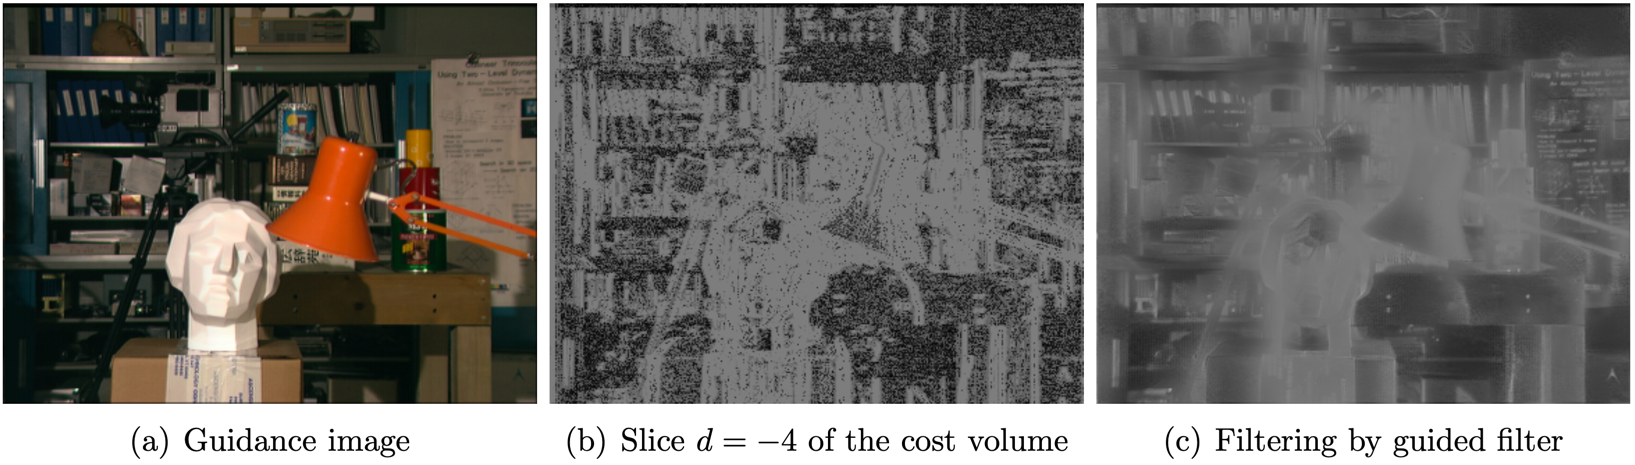
\includegraphics[width=0.9\textwidth]{assets/stereomatching/guidedfiltering}
    \caption{The guided filter (figure from~\citep{stereomatching}).}
    \label{fig:sm_guidedfilter}
\end{figure}

For all pixel $i$ in the image, the filter considers a window around $i$ of a certain radius and uses information from
the original \enquote*{guidance} image (the left input image) to denoise the considered slice of the cost volume.
Hence, for each value of $d$, we can define the \textit{filtered} cost to be $C^{\text{filt}}(i,d)$, the value of the
pixel corresponding to pixel $i$ in the $d$th slice of the filtered cost volume.

In particular, the disparity value that is returned for a pixel $i$ is:
\[d(i)=\argmin_{d'\in [d_{\min},d_{\max}]}\left\{C^{\text{filt}}(i,d')\right\}\]

The authors finally check if the disparity found is constistent: the disparity from the left to the right image is
rejected if the disparity of the corresponding pixel in the right image is different.
That is, the disparity is rejected if the map from the left to the right image disagrees on the disparity with the
map from the right to the left image or if (for $d'(i)$ the disparity of pixel $i$ from right to left):
\[d(i)\neq -d'(i+d(i))\]

\begin{figure}[H]
    \centering
    \captionsetup{justification=centering}
    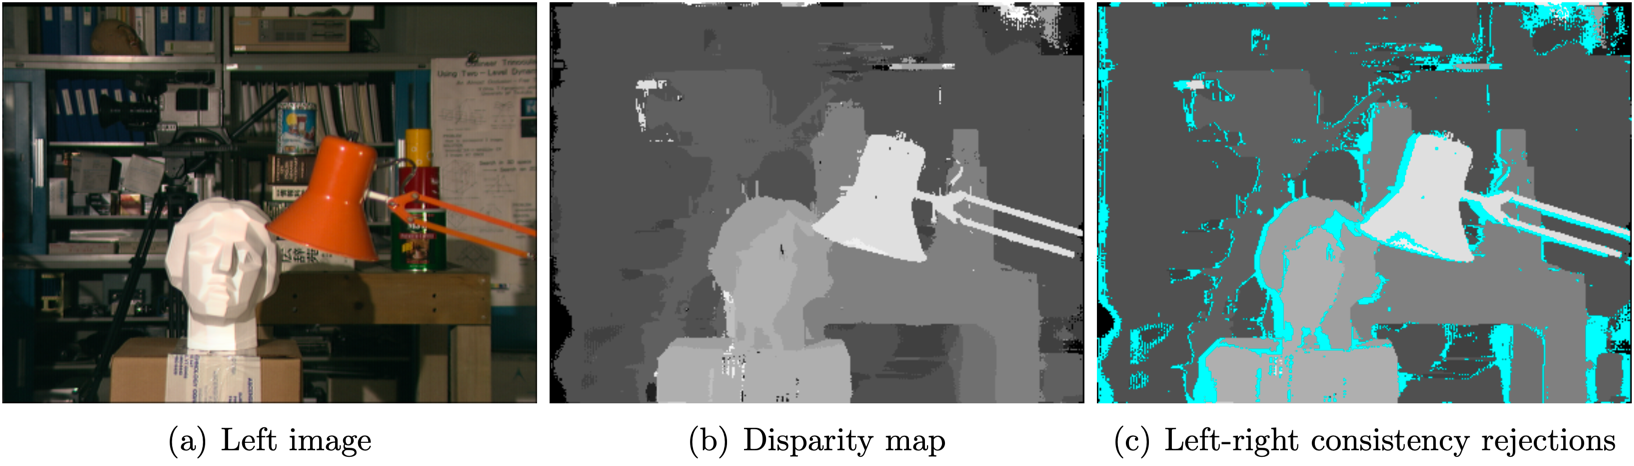
\includegraphics[width=0.9\textwidth]{assets/stereomatching/leftrightconsistency}
    \caption{Left-right consistency rejections (figure from~\citep{stereomatching}).}
    \label{fig:sm_leftrightconsistency}
\end{figure}

In particular, pixels representing occluded points in either image will necessarily be rejected.
It could also happen that a disparity value is rejected on textureless regions, where multiple pixels in the right
image could correspond to the pixel we are looking for in the left image.
To do inpainting, we consider a square window $\omega_i$ or a certain radius around the occluded pixel $i$.
The authors propose the following weight function, that is bigger for disoccluded points $j$ spatially close to $i$ and
for $j$ with a color close to the color of $i$ ($w_s,w_c$ are chosen weights):
\[W_{ij}=e^{-\frac{\left\|i-j\right\|^2}{w_s^2}}\cdot
e^{-\frac{\left\|I_{L,\text{filt}}(i)-I_{L,\text{filt}}(j)\right\|^2_c}{w_c^2}}\]
Then, they define the function $h(d)$ that simply sums all the weights of points $j$ in the window that are at a depth
at most $d$.
\[h(d)=\sum_{j\in\omega_i,d(j)\leq d} W_{ij} \]
Notice that in particular, $h(d)\leq h(d+1)$ for all $d$ (which means that taking the $d$ that maximizes $h$ does not
make any sense).
The value of $d$ that is chosen for occluded $i$ is the one that gives the median of $h$.
This means that if most of the weight is around some depth $d^*$, then a disparity value close to $d^*$ will be chosen
(which makes sense since we have high weights for pixels close in color and in space, we expect the disparity of the
occluded point to be close to the one of these pixels, \textit{QS.5}).

\begin{figure}[ht]
    \centering
    \captionsetup{justification=centering}
    \begin{minipage}{.5\textwidth}
        \centering
    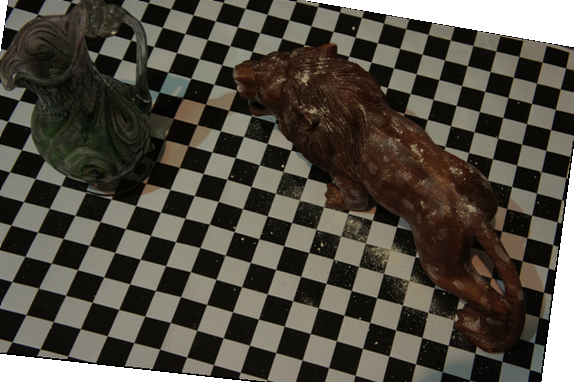
\includegraphics[width=0.7\textwidth]{assets/stereomatching/rect_lion_left}
    \end{minipage}%
    \hfill
    \begin{minipage}{.5\textwidth}
        \centering
    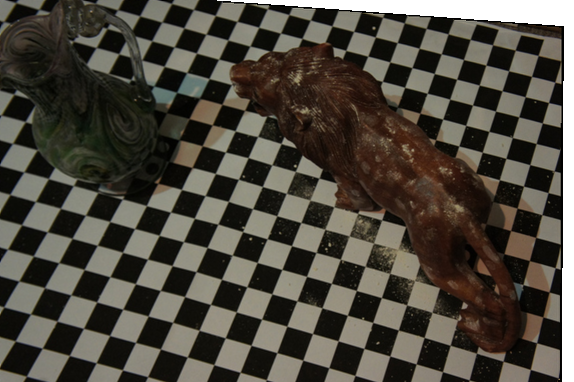
\includegraphics[width=0.7\textwidth]{assets/stereomatching/rect_lion_right}
    \end{minipage}
    \caption{Rectified left and right input images.}
    \label{fig:sm_input}
\end{figure}

We have run the online demo of paper~\citep{stereomatching} on the (rectified) images of figure~\ref{fig:sm_input}.
Figure~\ref{fig:sm_output} shows the output of the algorithm along with the occlusion map and an alternative result
of the algorithm with a simpler inpainting algorithm, where the final disparity value for an occluded pixel $i$ is
the disparity value of the first disoccluded pixel straight to the left or to the right.

\begin{figure}[ht]
    \centering
    \captionsetup{justification=centering}
    \begin{minipage}{.33\textwidth}
        \centering
    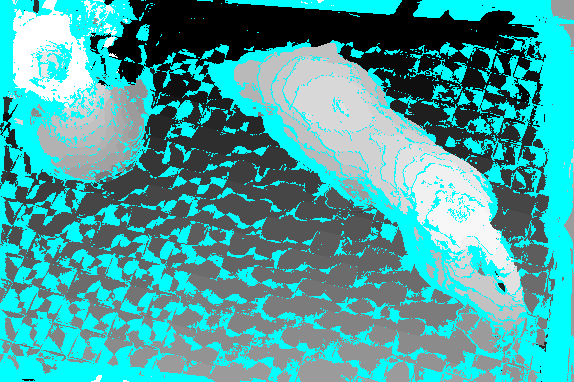
\includegraphics[width=0.95\textwidth]{assets/stereomatching/occlusion_map}
    \end{minipage}%
    \hfill
    \begin{minipage}{.33\textwidth}
        \centering
    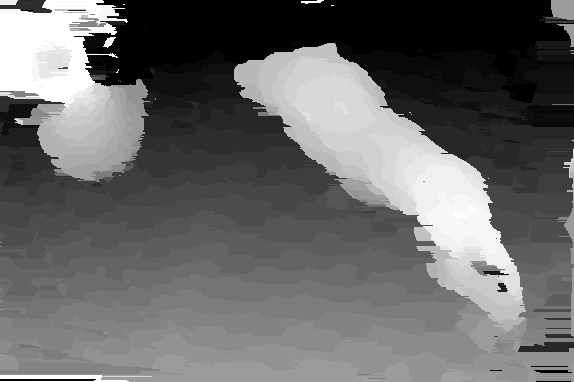
\includegraphics[width=0.95\textwidth]{assets/stereomatching/simple_filling}
    \end{minipage}%
    \hfill
    \begin{minipage}{.33\textwidth}
        \centering
    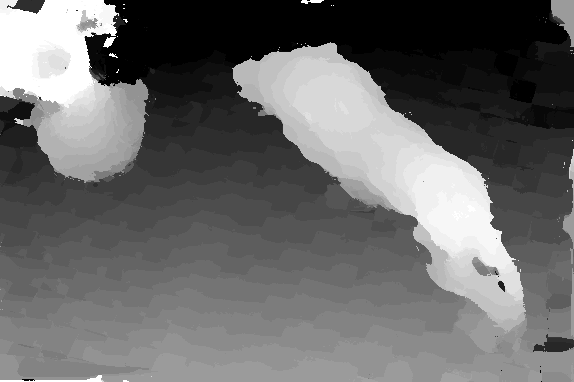
\includegraphics[width=0.95\textwidth]{assets/stereomatching/disparity_map_out}
    \end{minipage}
    \caption{Outputs of the stereo matching of figure~\ref{fig:sm_input}.
    The map with the occluded pixels in blue is on the left, the map after a simple example fill in the center and the
    final map on the right.}
    \label{fig:sm_output}
\end{figure}

We can observe in figure~\ref{fig:sm_output} that a lot of pixels that are not occluded in either images have their
disparity value rejected.
This is because the checkerboard does not have a lot of texture and many parts are monochrome.
In monochrome regions, a large range of disparity values are possible for these pixels and there is no
reason that the disparity values found from left to right and from right to left are the same.

The output map is a disparity map and not a depth map, since the pixels closer to the camera are white (and are thus
of higher value, \textit{QS.2}).
Notice that the disparity map is of poor quality along the (especially right) border of the map.
This is because there are no pixels that represent the same actual point in the right image (\textit{QS.1}).

We can observe that the handle of the vase is not correctly detected by the stereo matching algorithm.
This could be explained by the non-lambertian nature of said handle (and the whole vase in general).
The inner part of the handle is very reflective, which could easily break the algorithm.
The left side of the vase is also badly reconstructed in the disparity map because it is cut off in the
right image: it is on the very border of the image (\textit{QS.3}).

Take a look at section~\ref{subsec:viewsynthesis} and~\ref{subsec:icp} for results with our own figures (\textit{QS.4}).

\newpage
\section{Second Part}\label{sec:secondpart}

    \subsection{View Synthesis}\label{subsec:viewsynthesis}

View synthesis is a technique used to generate views between two input views.
Figures~\ref{fig:vs_left_input} and~\ref{fig:vs_right_input} give the two input images and their associated disparity
map (generated with~\citep{stereomatching}).
We implemented view synthesis with the assumption that the two camera positions differ only by a $x$-translation
($R=I,t=\left[x\hspace*{2mm} 0\hspace*{2mm} 0\right]^t $).

\begin{figure}[ht]
    \centering
    \captionsetup{justification=centering}
    \begin{minipage}{.5\textwidth}
        \centering
    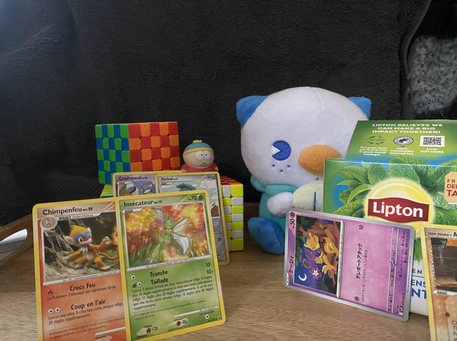
\includegraphics[width=0.7\textwidth]{assets/viewsynthesis/left_rect}
    \end{minipage}%
    \hfill
    \begin{minipage}{.5\textwidth}
        \centering
    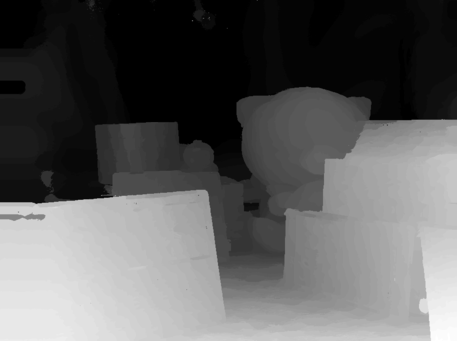
\includegraphics[width=0.7\textwidth]{assets/viewsynthesis/disparity_map_left}
    \end{minipage}
    \caption{The left input view with the associated disparity map.}
    \label{fig:vs_left_input}
\end{figure}

\begin{figure}[ht]
    \centering
    \captionsetup{justification=centering}
    \begin{minipage}{.5\textwidth}
        \centering
    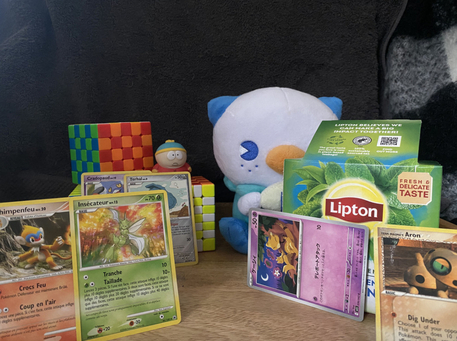
\includegraphics[width=0.7\textwidth]{assets/viewsynthesis/right_rect}
    \end{minipage}%
    \hfill
    \begin{minipage}{.5\textwidth}
        \centering
    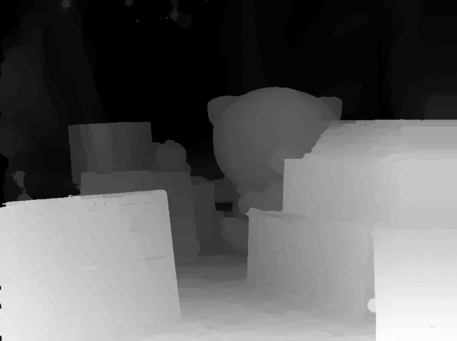
\includegraphics[width=0.7\textwidth]{assets/viewsynthesis/disparity_map_right}
    \end{minipage}
    \caption{The right input view with the associated disparity map.}
    \label{fig:vs_right_input}
\end{figure}

Given the two images and their respective disparity map, it is easy to build a new image that is located at the
point $0<\alpha<1$ between the two images ($\alpha=0$ corresponds to the left image, $\alpha=1$ corresponds to the
right image and $\alpha=1/2$ corresponds to the view exactly in the middle of the two shots).
For all pixels $(i,j)$ in the left image, we know that it would land at position $(i-\alpha d,j)$ for view $\alpha$ if
the disparity was $d$ ($d>0$).
Doing this for all pixels in the image, we get a barebones version of view $\alpha$.
If two pixels land on the same pixel in the output image, we keep the one with the highest disparity (since it's the
one with the smallest depth and therefore should appear in front of the other).
If this happens, we necessarily will have empty pixels in the output image.
Empty pixels can also appear because of disocclusions.
To fill in (not necessarily all) empty pixels, we can build another output image but this time using only the right
image as a base, where pixel $(i,j)$ is mapped to pixel $(i+\alpha d,j)$ in the output image.

The above method is known as forwards view synthesis.

It could still be the case that some pixels are left empty by this method.
In this case, we can use backwards view synthesis.
The idea of this method is, instead of projecting the pixels into the output image, look for every pixel in the output
image which pixel lands the closest.
We again do this process from left to right and from right to left.
Merging the two images is not as trivial as before since all pixels are filled: we cannot simply discard the pixel that
is empty, we always have two candidates.
To solve this issue, we can attribute a score to each pixel in the two generated images and keep the pixel with the
better score.
The score is the distance between the pixel and the position where the pixel that was mapped to it fell.
That is, if there is a pixel at position $(i,j)$ in the output image that came from a pixel $(i',j)$ with disparity $d$,
the score for $(i,j)$ is $|i-(i'+\alpha d)|$.

The code that handles forwards and backwards view synthesis can be found in function the \texttt{render\_one} of
\texttt{view\_synthesis/src/view\_synthesizer/ViewSynthesizer.py} (\textit{QV.1}).

To apply everything on our test images, we had to take pictures of a scene while being careful to only move the camera
in the $x$-axis.
We achieved this using a ruler and a lego rail.
The images were then corrected for radial distortion and rectified
(since it is virtually impossible to get a true $x$-translation of the camera).
The two disparity maps were obtained using the IPOL paper~\citep*{stereomatching} (after tweaking the parameters).
The images were then cropped to remove the empty pixels that came from the rectification.
Finally, the disparity maps were cleaned by hand, to finally obtain the result of figure~\ref{fig:vs_cleaned_disp}
(there were visible artifacts as well as blatantly wrong disparities for certains regions of the images
as we can see in figure~\ref{fig:vs_left_input} and~\ref{fig:vs_right_input}).

\begin{figure}[ht]
    \centering
    \captionsetup{justification=centering}
    \begin{minipage}{.5\textwidth}
        \centering
    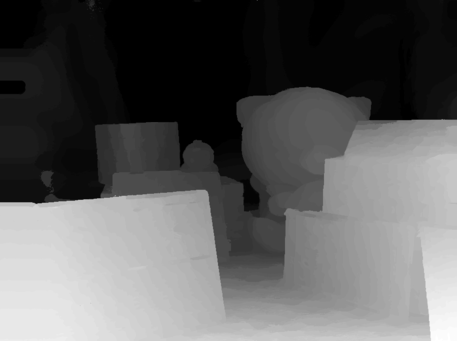
\includegraphics[width=0.7\textwidth]{assets/viewsynthesis/disparity_map_left_clean}
    \end{minipage}%
    \hfill
    \begin{minipage}{.5\textwidth}
        \centering
    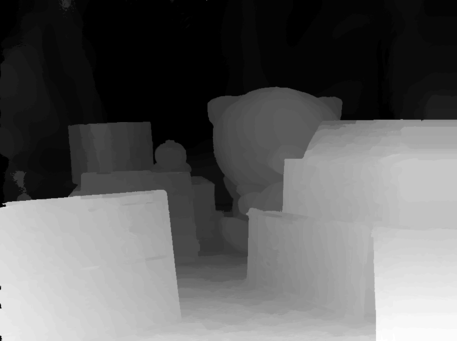
\includegraphics[width=0.7\textwidth]{assets/viewsynthesis/disparity_map_right_clean}
    \end{minipage}
    \caption{The cleaned-up disparity maps.}
    \label{fig:vs_cleaned_disp}
\end{figure}

\begin{figure}[ht]
    \centering
    \captionsetup{justification=centering}
    \begin{minipage}{.5\textwidth}
        \centering
    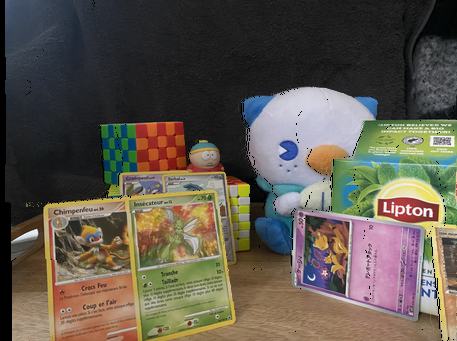
\includegraphics[width=0.95\textwidth]{assets/viewsynthesis/image_11_forwards}
    \end{minipage}%
    \hfill
    \begin{minipage}{.5\textwidth}
        \centering
    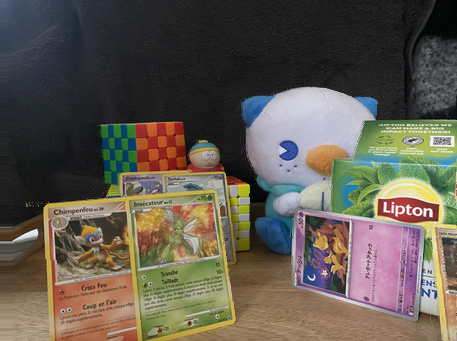
\includegraphics[width=0.95\textwidth]{assets/viewsynthesis/image_11_backwards}
    \end{minipage}
    \caption{The synthesized view point using forwards (left) and backwards (right) view synthesis.}
    \label{fig:vs_forward_backward}
\end{figure}

Performing view synthesis to generate a certain number of viewpoints between the two reference images is easy, and all
that is left to do is to build a quilt and project it on a lenticular display.
We generate a quilt of size $11\times 6$ and thus synthesize $66$ images.
Experimentally, we found that only varying $\alpha$ uniformly between 0 and 1 did not yield a large enough parallax
effect.
Hence, we decided to create 66 images for a varying $\alpha$ between $-0.6$ and $1.6$.
The images generated for values of $\alpha$ outside the regular range ($[0,1]$) are necessarily of lesser quality than
the others because they correspond to viewpoints ever more to the left than the left input image (or to the right
than the right input image), but it does not really matter on small screens and the effect is still quite convincing.

We observe that there are small artifacts in the output views, which we believe are caused by rescaling artifacts in
the disparity maps (the images were too big to be processed and had to be scaled down) as well as the manual cleanup
(which was done by mostly eyeballing both the edges of objects and the disparity).

The full source code associated to this section, as well as the generated images, the generated quilt and a video
of the lenticular display are provided alongisde this report (\textit{QV.2}).

PSNR is a measure of the quality of a reconstructed image.
We have taken a picture of the scene at the halfway point between the left and right images.
This gives a reference image $R$.
For a generated image $I$, the PSNR for a component $c$ (like a specific color channel) is computed as follows,
for a bit depth $b$:
\begin{gather*}
    \text{MSE}_c=\frac{1}{mn}\sum_{i=1}^{n} \sum_{j=1}^{m} [R(i,j)_c-I(i,j)_c]^2\\
    \text{PSNR}_c=10\log_{10}\left(\frac{(2^b-1)^2}{\text{MSE}_c}\right)
\end{gather*}
On the pair of images of figure~\ref{fig:vs_output}, we find a PSNR value of $20.25 dB$, which is relatively poor.
This is easily explained by the fact that the two images slightly differ in camera position (it is clear when
superposing the two images and alternating between them).

\begin{figure}[ht]
    \centering
    \captionsetup{justification=centering}
    \begin{minipage}{.5\textwidth}
        \centering
    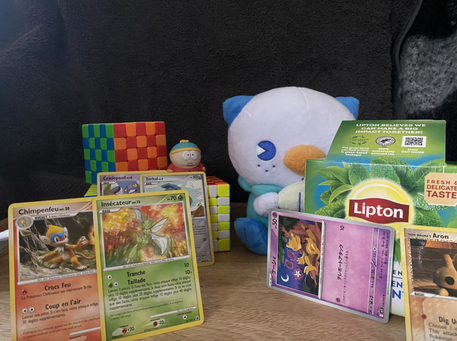
\includegraphics[width=0.95\textwidth]{assets/viewsynthesis/mid_rect}
    \end{minipage}%
    \hfill
    \begin{minipage}{.5\textwidth}
        \centering
    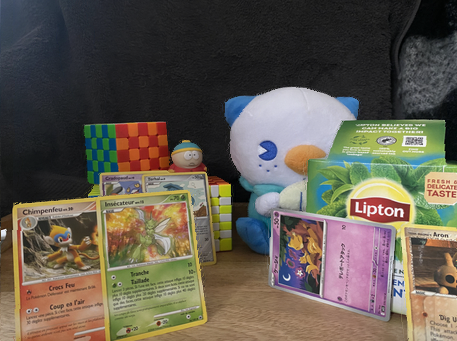
\includegraphics[width=0.95\textwidth]{assets/viewsynthesis/image_30_backward}
    \end{minipage}
    \caption{The true mid-view (left) and the equivalent view generated using backwards view synthesis (right).}
    \label{fig:vs_output}
\end{figure}

IV-PSNR~\citep{ivpsnr} is an equivalent to PSNR but for immersive video (hence the \enquote*{IV} prefix).
The idea is very similar to the regular PSNR except that the corresponding pixel in the generated image $I$ is taken to
be the best candidate in a square window of radius $B$, instead of having to be exactly $(i,j)$:
\[\text{IV-MSE}_c=\frac{1}{mn}\sum_{i=1}^{n} \sum_{j=1}^{m} \min_{\substack{i-B\leq i'\leq i+B\\j-B\leq j'\leq j+B}}
[R(i,j)_c-I(i',j')_c+\text{GCD}_c]^2\]
Where $B$ is the width of a window and $\text{GCD}_c$ is the average global component difference:
\[\text{GCD}=\frac{1}{mn}\sum_{i=1}^{n} \sum_{j=1}^{m}[R(i,j)_c-I(i,j)_c]\]
This gives a more way of computing the PSNR for videos or for synthesized images with slight pixel translations that
are usually not noticeable.
As a sidenote, the IV-PSNR is not symmetric as-is ($R$ and $I$ are not interchangeable and
to make it symmetric, it could be evaluated as the minimum of the IV-PSNR in both directions).

The authors of~\citep{ivpsnr} have provided a tool that can be used to compute the IV-PSNR easily, available
at~\url{https://github.com/jstankowski/ivpsnr}.
This tool computes both the PSNR and the IV-PSNR (as well as the WS-PSNR and the IV-SSIM).
The computed value for the IV-PSNR is $32.08 dB$, which is good (\textit{QV.3}).

    \subsection{Iterated Closest Point}\label{subsec:icp}

ICP is a technique used to align two point clouds to either create a denser one or stitch two mostly disjoint
point clouds into one.

Assuming that we have two roughly aligned points clouds $A$ and $B$, we will select a subset of matching points $A'$ and
$B'$ such that $A'_i$ corresponds to $B'_i$ (that are both close in distance and in color).
Then, we optimize the following function to find a rotation $R^*$ and a translation $t^*$ that make the matching pairs
of points overlap even more:
\[R^*, t^*=\argmin_{R,t}\sum_{i} \left\|A'_i-(RB'_i+t)\right\|_2^2\]
We then apply the found rotation and translation to update the set $B$: $B\leftarrow R^* B+t^*$.
Then, we can find a new set of matching points and repeat until convergence.

We have taken four pictures of our subject (two on the right and two on the left), rectified them
using the IPOL paper~\citep{rectification} and generated the two corresponding disparity maps using another IPOL
paper~\citep{stereomatching}.
As another preprocessing step, we removed the background of our input images manually using Apple's isolate subject
feature\footnote{\url{https://support.apple.com/en-gb/guide/photos/pht53d914053/mac}}.
Having the background in the point clouds could make the process of ICP harder, and we only require a 3D point cloud of
the subject anyway.
The results of this first step can be seen in figure~\ref{fig:icp-input}.
As we can see, the disparity maps are bad for the background, which is a non-issue.

\begin{figure}[ht]
    \centering
    \captionsetup{justification=centering}
    \begin{minipage}{.25\textwidth}
        \centering
    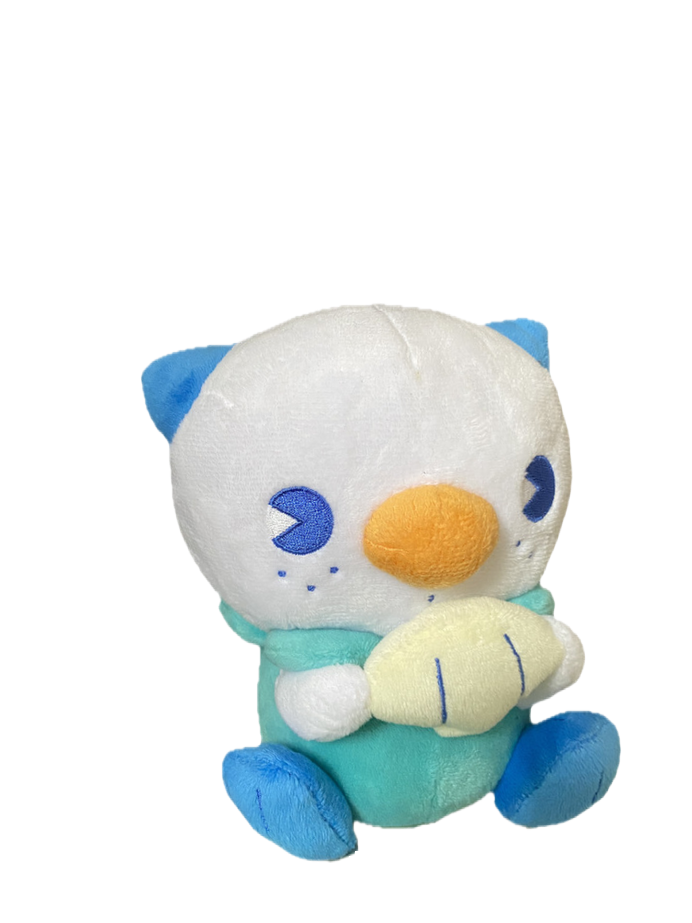
\includegraphics[width=0.95\textwidth]{assets/icp/rect_left}
    \end{minipage}%
    \begin{minipage}{.25\textwidth}
        \centering
    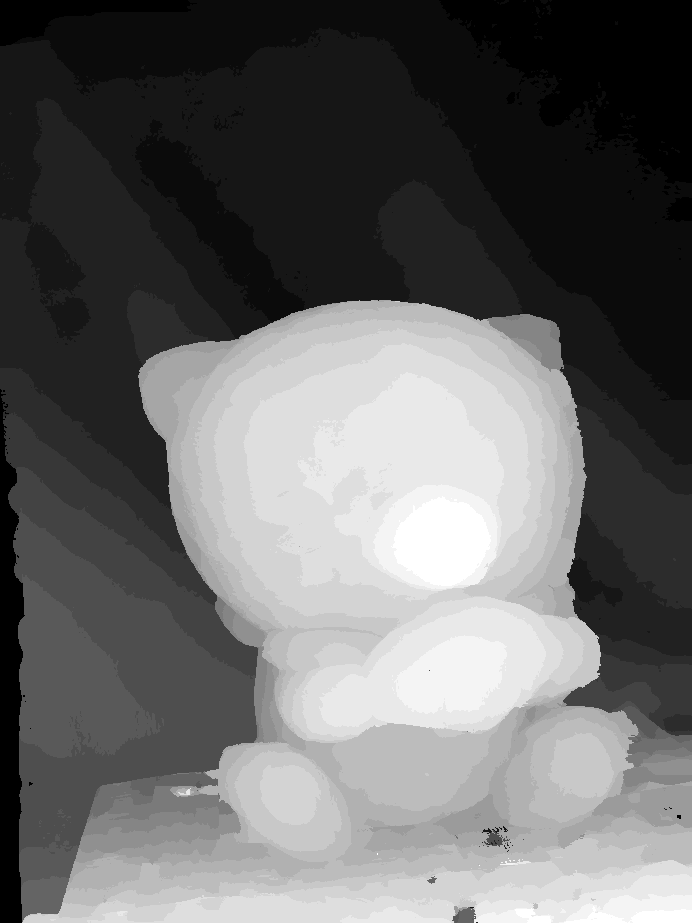
\includegraphics[width=0.95\textwidth]{assets/icp/depth_left}
    \end{minipage}%
    \begin{minipage}{.25\textwidth}
        \centering
    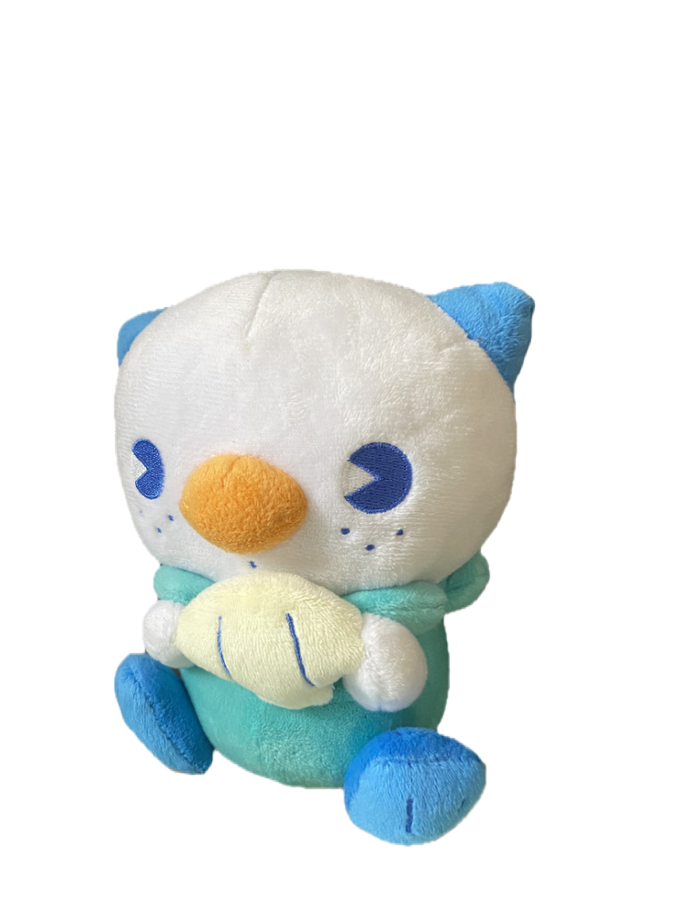
\includegraphics[width=0.95\textwidth]{assets/icp/rect_right}
    \end{minipage}%
    \hfill
    \begin{minipage}{.25\textwidth}
        \centering
    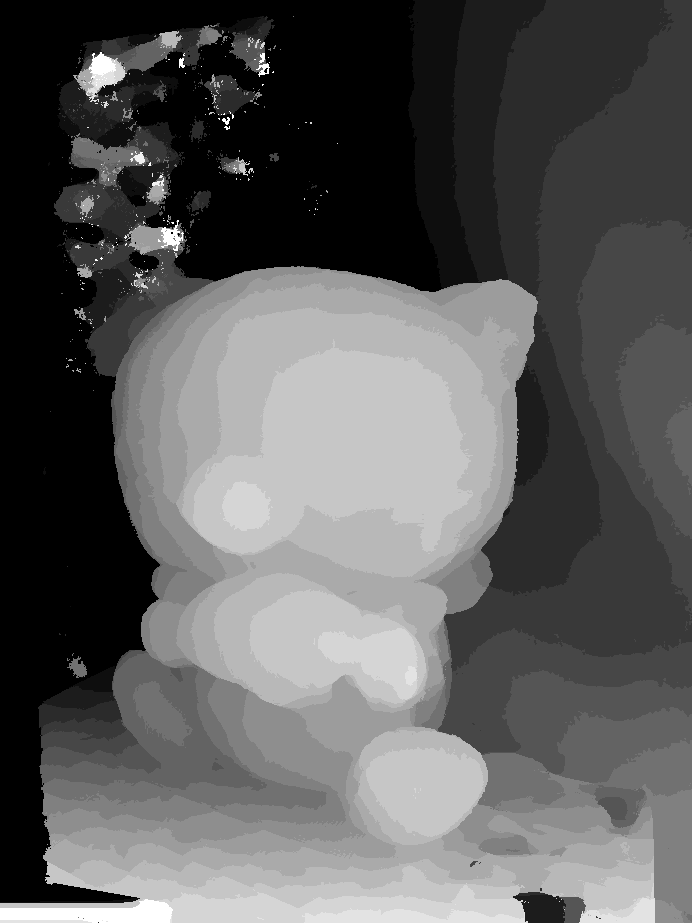
\includegraphics[width=0.95\textwidth]{assets/icp/depth_right}
    \end{minipage}
    \caption{The left and right images with their respective disparity maps.}
    \label{fig:icp-input}
\end{figure}

We can easily project points in 3D space and create a point cloud with the equations of section~\ref{subsec:rectification},
such as~\eqref{eq:disparitydepth} (with $f\approx 730$ as estimated previously).
Since the disparity maps are discrete by nature, projecting points in 3D space will create sort of a layered point
cloud, as can be seen in the leftmost image of figure~\ref{fig:icp-pcs}.

Then, using Meshlab~\citep{meshlab}, we were able to import the two point clouds, remove isolated points
and merge them using their implementation of ICP\@.
We first did a manual rough registration step by matching pairs of corresponding points to get a first alignment and
then ran the algorithm (\textit{QP.1}).
Since ICP only changes the alignment of the two point clouds, it can not change the position of each voxel individually
and the result looks like what is shown in figure~\ref{fig:icp-pcs} (middle and right images).
If we look at the middle image, we can see the two layered point clouds overlapping.
The rightmost image gives a midpoint view, which looks improvable.

\begin{figure}[ht]
    \centering
    \captionsetup{justification=centering}
    \begin{minipage}{.33\textwidth}
        \centering
    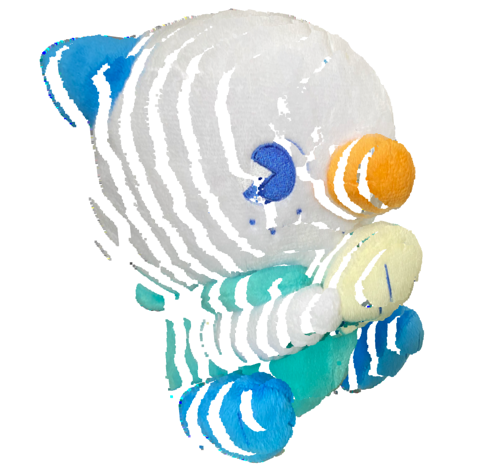
\includegraphics[width=0.95\textwidth]{assets/icp/left_pc}
    \end{minipage}%
    \begin{minipage}{.33\textwidth}
        \centering
    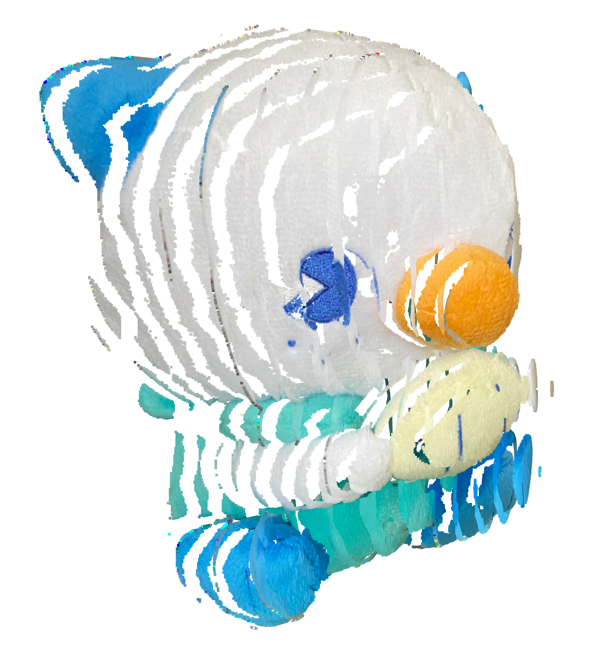
\includegraphics[width=0.95\textwidth]{assets/icp/out_left}
    \end{minipage}%
    \begin{minipage}{.33\textwidth}
        \centering
    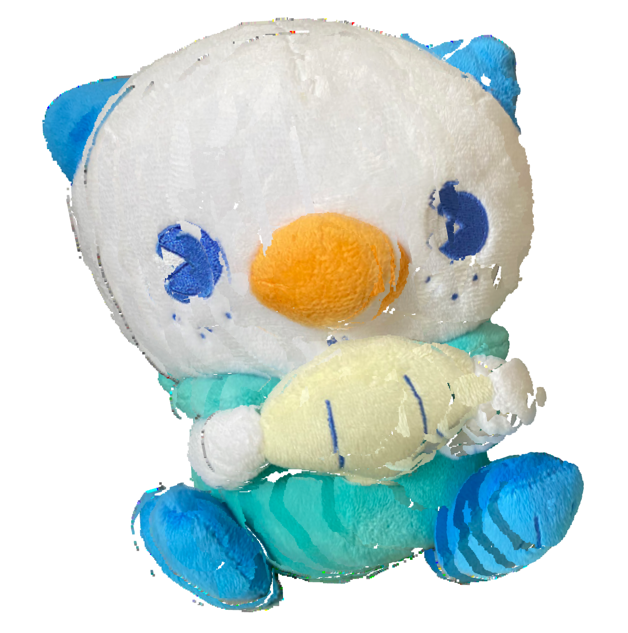
\includegraphics[width=0.95\textwidth]{assets/icp/out_mid}
    \end{minipage}
    \caption{The left image projected in 3D (left) and the final merged point cloud from the left (middle) and from
    the center (right image).}
    \label{fig:icp-pcs}
\end{figure}

To remedy the layered point cloud issue, we use a filtered version of the disparity maps generated with a bilateral
filter (with parameters found by trial and error) in order to project the images in 3D space.
This gives smoother point clouds, more suited for our purposes.
Figure~\ref{fig:icp-pcs_gaussed} shows the point cloud generated from the left input image and the final point cloud
glued using ICP in Meshlab (\textit{QP.2}).

\begin{figure}[ht]
    \centering
    \captionsetup{justification=centering}
    \begin{minipage}{.33\textwidth}
        \centering
    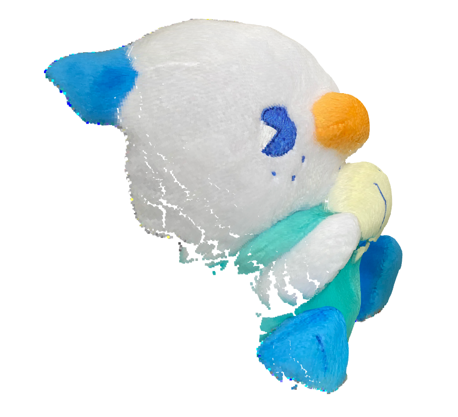
\includegraphics[width=0.95\textwidth]{assets/icp/left_pc_gauss}
    \end{minipage}%
    \begin{minipage}{.33\textwidth}
        \centering
    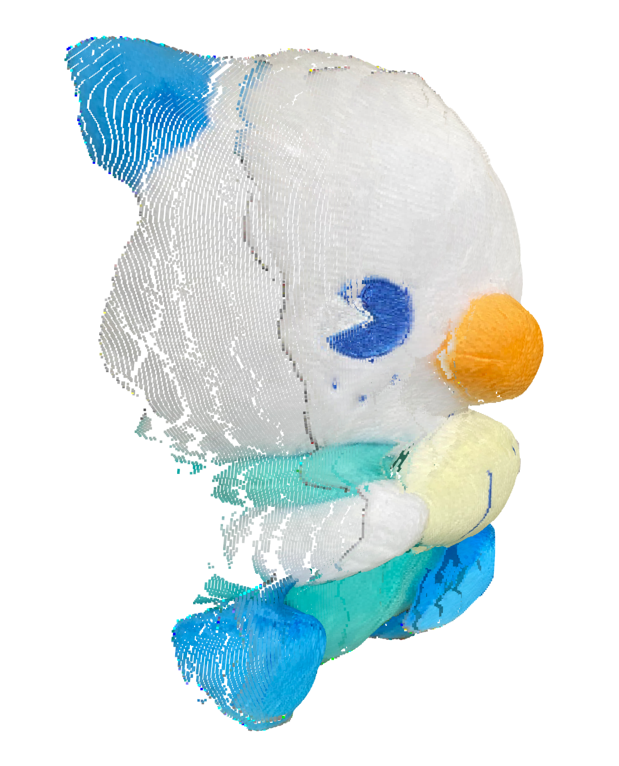
\includegraphics[width=0.95\textwidth]{assets/icp/out_gauss_left}
    \end{minipage}%
    \begin{minipage}{.33\textwidth}
        \centering
    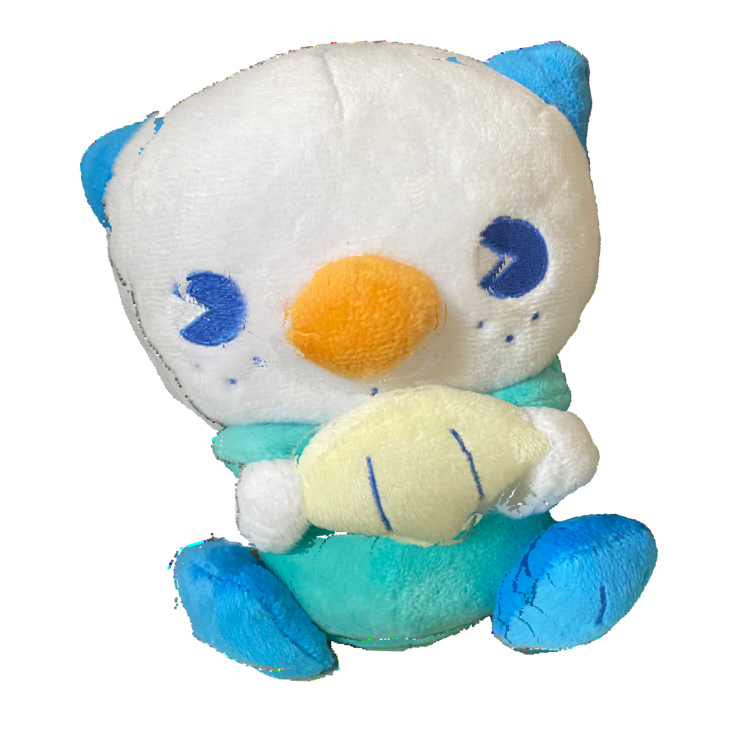
\includegraphics[width=0.95\textwidth]{assets/icp/out_gauss_mid}
    \end{minipage}
    \caption{The left image projected in 3D (left) and the final merged point cloud from the left (middle) and from
    the center (right image), generated using a filtered version of the disparity maps.}
    \label{fig:icp-pcs_gaussed}
\end{figure}

The code used for this section as well as the input images and the various point clouds (input and output to ICP) are
provided alongside this document (\textit{QP.3}).

    \subsection{Colmap}\label{subsec:colmap}

\question{Report (provide a trend on) how the quality of the reconstruction changes with the number of photos used in
the processing. How many input pictures (order of magnitude) are needed to reconstruct your 3D scene decently?}

\question{Report intrinsics $K$ and extrinsics $(R|t)$ between the first and $N$-th input view, with $N$ in the order
of ¼ of the total number of input views you used for the 3D reconstruction. Also provide radial distortion parameters.
Do all these values look reasonable to you?}

\question{Extract and show the depth map for one view.}

\question{Redo the previous two exercises using Colmap, instead.}


    \subsection{Zhang's method}\label{subsec:zhangsmethod}

\question{Which initial guess is given to the SfM in [Y,Z]? Explain how it is obtained.}

\question{Find the correspondences between the theory syllabus text and the [Y,Z] references to explain the main
processing steps. Your description can refer to page numbers and equations in the syllabus
    (consider this question rather as preparation for similar questions at the oral exam; do not give too many
    details in the report).}

\question{Is radial distortion estimation (and removal) embedded as with SfM from the theory lessons? Explain the
similarities and/or differences.}


    \bibliography{refs}
    
\end{document}